\graphicspath{{Einstieg/eps/}} \cleardoublepage
%%%%%%%%%%%%%%%%%%%%%%%%%%%%%%%%%%%%%%%%%%%%%%%%%%%%%%%%%%%%%%%%%%%%%%%%%%%%%%%%%%%%%%%%%%%%%%%%%%%%%%%%%%%%%%%%%%%%%%%%%%%%

\chapter{Der Einstieg in die Handhabung}
\label{Einstieg}

%%%%%%%%%%%%%%%%%%%%%%%%%%%%%%%%%%%%%%%%%%%%%%%%%%%%%%%%%%%%%%%%%%%%%%%%%%%%%%%%%%%%%%%%%%%%%%%%%%%%%%%%%%%%%%%%%%%%%%%%%%%%

Im folgenden werden die einzelnen Funktionen von \wspwin{} n\"{a}her erl\"{a}utert. Die Ausf\"{u}h\-rungen orientieren sich an der
Men\"{u}struktur des Programms. Diese ist entsprechend der im Rahmen einer Spiegellinienberechnung nacheinander auszuf\"{u}hrenden
Arbeitsschritte aufgebaut. Das bedeutet, da{\ss} das Programm von links nach rechts in der Men\"{u}leiste durchzuarbeiten ist.

So wird zuerst ein Projekt angelegt, danach eine Zustandsdatei und schlie{\ss}lich werden Profile erstellt und bearbeitet.
Anschlie{\ss}end ist eine Abflu{\ss}datei zu erzeugen (Randbedingungen), bevor im letzten Schritt die eigentliche Berechnung
ausgef\"{u}hrt werden kann. Um das Arbeiten mit \wspwin{} zu erlernen, sollten Sie die nachfolgend erl\"{a}uterten
Programmoptionen, wie beschrieben, durcharbeiten. Dabei ist es sinnvoll, zun\"{a}chst alle als Zusatzoptionen in den
nachfolgenden Kapiteln aufgef\"{u}hrten Funktionen auszulassen und diese erst n\"{a}her zu betrachten, nachdem einmal eine
komplette Berechnung durchgespielt wurde.


%%%%%%%%%%%%%%%%%%%%%%%%%%%%%%%%%%%%%%%%%%%%%%%%%%%%%%%%%%%%%%%%%%%%%%%%%%%%%%%%%%%%%%%%%%%%%%%%%%%%%%%%%%%%%%%%%%%%%%%%%%%%
\section{Das Starten des Programms}
%%%%%%%%%%%%%%%%%%%%%%%%%%%%%%%%%%%%%%%%%%%%%%%%%%%%%%%%%%%%%%%%%%%%%%%%%%%%%%%%%%%%%%%%%%%%%%%%%%%%%%%%%%%%%%%%%%%%%%%%%%%%

Nach der Installation kann das Programm durch Aktivierung des Programmsymbols \menu{Spiegellinienberechnung} im Startmen\"{u}
der Task-Leiste aktiviert werden. Hier finden sich zwei Untermen\"{u}punkte \menu{\marrow WSPWIN} zum Starten und
\menu{\marrow UnInstallShield} zum L\"{o}schen des Programms.
\begin{figure}[hbt]
    \centering
    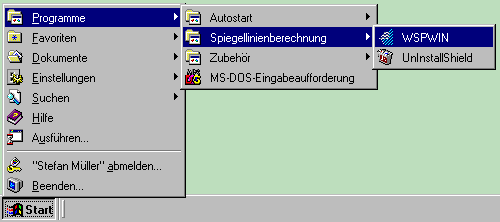
\includegraphics[width=0.8\textwidth]{Windows_Start}
    \caption{Programmstart unter Windows}
    \label{Einstieg Abb Programmstart}
\end{figure}


\clearpage
%%%%%%%%%%%%%%%%%%%%%%%%%%%%%%%%%%%%%%%%%%%%%%%%%%%%%%%%%%%%%%%%%%%%%%%%%%%%%%%%%%%%%%%%%%%%%%%%%%%%%%%%%%%%%%%%%%%%%%%%%%%%
\section{Projekte bearbeiten}
%%%%%%%%%%%%%%%%%%%%%%%%%%%%%%%%%%%%%%%%%%%%%%%%%%%%%%%%%%%%%%%%%%%%%%%%%%%%%%%%%%%%%%%%%%%%%%%%%%%%%%%%%%%%%%%%%%%%%%%%%%%%

\begin{figure}[ht]
   \centering
   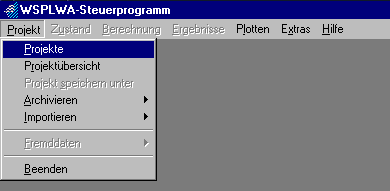
\includegraphics{MenueProjekte}
   \caption{Der Men\"{u}punkt Projekt}
   \label{Einstieg Abb MenueProjekt}
\end{figure}


\subsection{Ein neues Projekt anlegen}

Nach dem Start des Programms gelangen Sie \"{u}ber das Men\"{u} \menu{\marrow \underline{P}rojekt \marrow \underline{P}rojekte} in
die \dialog{Projektauswahlmaske} (Abbildung~\ref{Einstieg Abb Projektauswahlmaske}). Sie m\"{u}ssen nun zun\"{a}chst ein
bestehendes Projekt \"{o}ffnen oder ein neues Projekt, d.h. Verzeichnis, erstellen. In diesem Verzeichnis werden alle
nachfolgenden Arbeiten gespeichert. Bei sp\"{a}teren Arbeiten k\"{o}nnen Sie dann entscheiden, ob diese im selben Verzeichnis
abgelegt werden sollen (dann ist nur das bereits existierende Projekt zu \"{o}ffnen), oder ob sie f\"{u}r die neuen Arbeiten
wieder ein neues Verzeichnis einrichten m\"{o}chten.
\begin{figure}[hbt]
    \centering
    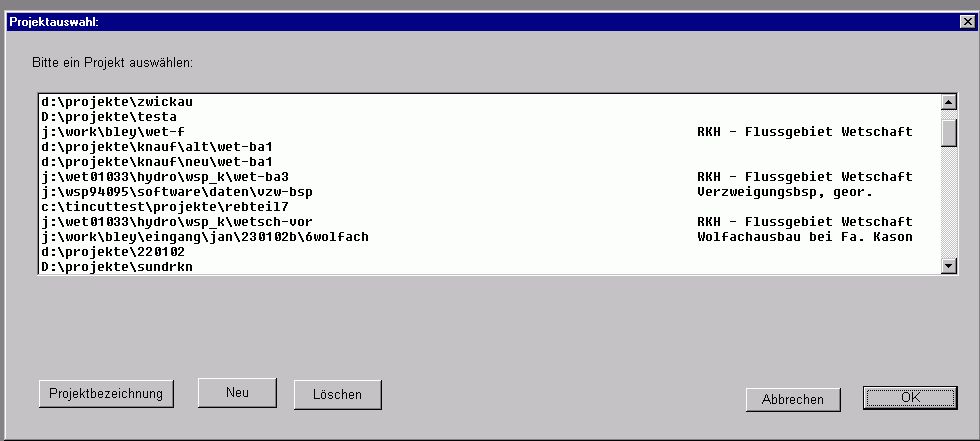
\includegraphics[width=1.0\textwidth]{Projektauswahl}
    \caption{Die Projektauswahlmaske}
    \label{Einstieg Abb Projektauswahlmaske}
\end{figure}

\"{U}ber die Schaltfl\"{a}che \schalter{Neu} gelangen sie in den Dialog zur Erstellung eines neuen Projektes
(Abbildung~\ref{Einstieg Abb ProjektErstellen}). Zu Ihrer Information ist im oberen Teil der Maske der Pfadname des
Verzeichnisses aufgef\"{u}hrt, in dem Sie zuletzt gearbeitet haben. Sie k\"{o}nnen unter dem Men\"{u}punkt \menu{\marrow
E\underline{x}tras \marrow \underline{O}ptionen} ein Hauptverzeichnis angeben, das Ihnen immer als
Standarddatenverzeichnis an dieser Stelle erscheint, um z.B. alle Projekte in einem extra \wspwin{}-Projektordner
abzulegen (siehe auch Abschnitt~\ref{Installation Subsec Verzeichnisse}).
\begin{figure}
    \centering
    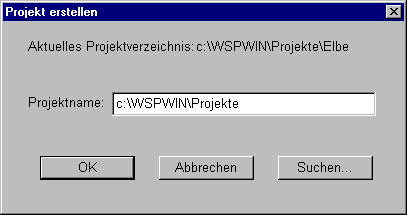
\includegraphics[width=0.6\textwidth]{ProjektErstellen}
    \caption{Anlegen eines neuen Projektes}
    \label{Einstieg Abb ProjektErstellen}
\end{figure}

Zum Anlegen eines neuen Projektordners geben sie den gew\"{u}nschten Pfad in das Eingabefeld ein und best\"{a}tigen die Eingabe
mit \schalter{OK}. Das neu erstellte Projekt erscheint nun in der \dialog{Projektauswahlmaske}. Ein Projekt stellt in
der Hierarchie der Dateiverwaltung die oberste Kategorie dar. S\"{a}mtliche weiteren Bearbeitungsschritte beziehen sich
anschlie{\ss}end auf das neu erstellte (bzw. ausgew\"{a}hlte) Projekt.
\begin{hinweis}
    In der Maske \dialog{Projekt erstellen}, die nach Bet\"{a}tigung der Schaltfl\"{a}che \schalter{Neu} aus der
    \dialog{Projektauswahlmaske} heraus erscheint, haben Sie auch die M\"{o}glichkeit \"{u}ber die Schaltfl\"{a}che \schalter{Suchen...}
    ein Verzeichnis \"{u}ber den Standard-Windows-Dialog im Verzeichnisbaum zu suchen.
    Im Anschlu{\ss} an die Selektion existierender Verzeichnisse k\"{o}nnen Sie im Editierfeld Verzeichnis ein oder mehrere
    Unterverzeichnisse angeben.
\end{hinweis}

\"{U}ber die Schaltfl\"{a}che \schalter{Projektbezeichnung} k\"{o}nnen sie jedem Projekt eine zus\"{a}tzliche Bezeichnung (maximal
60~Zeichen, Leerzeichen sind erlaubt) zuordnen. Diese Projektbezeichnung erscheint sp\"{a}ter auf dem Ausdruck Ihrer
Ergebnisdatei. Die Projektbezeichnung stellt f\"{u}r Sie auch eine M\"{o}glichkeit dar, Ihre Projekte unabh\"{a}ngig vom unter
Umst\"{a}nden nicht eindeutigen Pfadnamen leichter zu identifizieren.


\subsection{Projekt \"{o}ffnen}
\label{Einstieg Subsec ProjektOeffnen}

Wenn Sie den Men\"{u}punkt \menu{\marrow \underline{P}rojekt \marrow \underline{P}rojekte} gew\"{a}hlt haben, gelangen Sie
automatisch in die \dialog{Projektauswahlmaske}, aus der heraus ein Projekt auszuw\"{a}hlen bzw. zu \"{o}ffnen ist.

Wenn noch kein neues Projekt angelegt wurde, ist die Projektauswahlmaske leer, ansonsten werden alle verf\"{u}gbaren
Projekte aufgelistet. \"{U}ber den Schalter \schalter{OK} \"{o}ffnen Sie das markierte Projekt (vgl. Abbildung~\ref{Einstieg
Abb Projektauswahlmaske}). Ohne ein ge\"{o}ffnetes Projekt, k\"{o}nnen keine weiteren Arbeitsschritte ausgef\"{u}hrt werden. Alle
weiteren Arbeiten beziehen sich dann auf das ausgew\"{a}hlte Verzeichnis und werden in diesem abgespeichert. \"{U}ber die
Option \schalter{Projektbezeichnung} haben Sie die M\"{o}glichkeit, die Projektbezeichnung zu modifizieren (siehe auch
Abschnitt~\ref{Einstieg Subsec ProjektOeffnen}).


\subsection{Projekt l\"{o}schen}

Neben dem Anlegen eines neuen Projektes und dem \"{O}ffnen bereits existierender Projekte bietet die
\dialog{Projektauswahlmaske} auch die M\"{o}glichkeit, ein Projekt zu l\"{o}schen. Markieren Sie das zu l\"{o}schende Projekt in der
Auswahlliste und w\"{a}hlen Sie den Schalter \schalter{L\"{o}schen}. Es folgt eine Sicherheitsabfrage ob Sie wirklich das gesamte
Projekt l\"{o}schen m\"{o}chten. An dieser Stelle k\"{o}nnen Sie den L\"{o}schvorgang noch abbrechen.

Bitte beachten Sie, da{\ss} s\"{a}mtliche Dateien in den Unterverzeichnissen \datei{...\textbackslash prof} und
\datei{...\textbackslash dath} des entsprechenden Projekt-Verzeichnisses gel\"{o}scht werden. Existieren in dem
Projektverzeichnis zus\"{a}tzliche Dateien oder Verzeichnisse (z.B. vom Plotprogramm) bleiben diese vom L\"{o}schvorgang
unber\"{u}hrt. Beachten Sie weiterhin, da{\ss} das aktuelle Projektverzeichnis nicht gel\"{o}scht werden kann. Dies kann erst
erfolgen, wenn ein anderes Projekt ge\"{o}ffnet wurde. Sollte ein Verzeichnis nicht mehr existieren, kann nur der
Projekteintrag entfernt werden (vgl. \menu{\marrow \underline{P}rojekt \marrow \underline{I}mportieren \marrow
Projekteintrag \underline{l}\"{o}schen}).


\subsection{Beispiel}

Legen Sie das Projekt \afz{Beispiel} auf Ihrer Festplatte an. \"{O}ffnen Sie dazu zun\"{a}chst die Projektauswahlmaske
(Abbildung~\ref{Einstieg Abb Projektauswahlmaske}) \"{u}ber das Men\"{u} \menu{\marrow \underline{P}rojekt \marrow
\underline{P}rojekte}. Mit Hilfe der Schaltfl\"{a}che \schalter{Neu} gelangen sie in den Dialog zur Erstellung eines neuen
Projektes. Geben Sie hier Pfad und Verzeichnisnamen Ihres Projektes ein, z.B.
\begin{quote}
    \datei{C:\textbackslash WSPWIN \textbackslash Projekte\textbackslash Beispiel}
\end{quote}
und best\"{a}tigen die Eingabe mit \schalter{OK}. Das neu angelegte Projekt erscheint jetzt in der Projektauswahlmaske.
Markieren Sie es und \"{o}ffnen Sie das Verzeichnis mit Hilfe von \schalter{OK}.


\clearpage
%%%%%%%%%%%%%%%%%%%%%%%%%%%%%%%%%%%%%%%%%%%%%%%%%%%%%%%%%%%%%%%%%%%%%%%%%%%%%%%%%%%%%%%%%%%%%%%%%%%%%%%%%%%%%%%%%%%%%%%%%%%%
\section{Zustandsdatei bearbeiten}
%%%%%%%%%%%%%%%%%%%%%%%%%%%%%%%%%%%%%%%%%%%%%%%%%%%%%%%%%%%%%%%%%%%%%%%%%%%%%%%%%%%%%%%%%%%%%%%%%%%%%%%%%%%%%%%%%%%%%%%%%%%%

Sobald Sie ein Projekt ge\"{o}ffnet haben, erreichen Sie automatisch die n\"{a}chste Kategorie der Dateiverwaltung, die Zustands-
oder Vernetzungsdatei.
\begin{figure}[hptb]
    \centering
    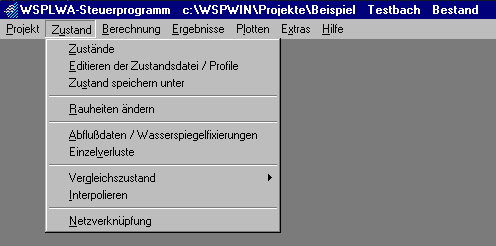
\includegraphics[width=0.7\textwidth]{MenueZustand}
    \caption{Das Men\"{u} Zustand}   \label{Einstieg Abb MenueZustand}
\end{figure}
Eine Zustandsdatei stellt die Verkn\"{u}pfung mehrerer Profildateien dar, die alle demselben geometrischen Zustand zugeh\"{o}rig
sind (z.B. Istzustand, Ausbauzustand, Bestand, Planung). Innerhalb eines Projektes k\"{o}nnen mehrere Zustandsdateien angelegt
werden, die ihrerseits wiederum unterschiedliche, aber auch gleiche Profile verwalten k\"{o}nnen.

\subsection{Eine neue Zustandsdatei anlegen}

Sofern Sie ein neues Projekt eingerichtet haben, sind in der Dialogmaske \dialog{Auswahl der Zustandsdatei} keine
Eintr\"{a}ge vorhanden. Um eine neue Zustandsdatei zu definieren, gelangen Sie \"{u}ber die Schaltfl\"{a}che
\schalter{Neue Zustandsdatei} in den Dialog \dialog{Neue Vernetzungsdatei anlegen}
(Abbildung~\ref{Einstieg Abb ZustandsdateiNeu}). Es erscheint eine Maske, die Sie zur Angabe des Gew\"{a}ssernamens, der Kennung
des Zustands, sowie des zuzuordnenden Datums auffordert.
\begin{hinweis}
   Vermeiden Sie beim Gew\"{a}ssernamen und Zustand Sonderzeichen, wie Punkt, Bindestrich, Unterstrich, Leerzeichen etc.,
   die bei sp\"{a}teren Bearbeitungsschritten zu Problemen f\"{u}hren k\"{o}nnen.
\end{hinweis}
Nachdem Sie eine neue Zustandsdatei erstellt haben, kehren Sie automatisch in die Maske zur\"{u}ck, in der Sie zur Auswahl
einer Vernetzungsdatei aufgefordert werden. Die neu erstellte Zustandsdatei wird nun aufgelistet.


\subsection{Zustandsdatei \"{o}ffnen}

Nach dem \"{O}ffnen eines Projektes werden Sie automatisch in die Dialogmaske gef\"{u}hrt, die Sie zur Auswahl einer Zustandsdatei
auffordert. In dieses Fenster gelangen Sie auch zu jedem anderen Bearbeitungszeitpunkt \"{u}ber den Men\"{u}punkt \menu{\marrow
Z\underline{u}stand \marrow \underline{Z}ust\"{a}nde}. S\"{a}mtliche Verkn\"{u}pfungsdateien innerhalb des Projektes werden
aufgelistet. Durch Markieren der gew\"{u}nschten Zustandsdatei (Mausklick auf den entsprechenden Listeneintrag) und
anschlie{\ss}endem Best\"{a}tigen mit \schalter{OK} w\"{a}hlen Sie eine Verkn\"{u}pfungsdatei aus.
\begin{figure}
   \centering
   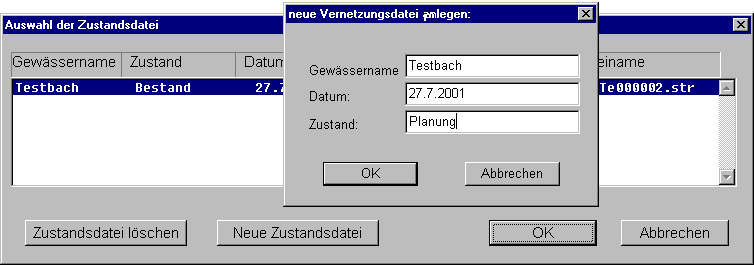
\includegraphics[width=0.9\textwidth]{NeuerZustand}
   \caption{Anlegen und \"{O}ffnen einer neuen Zustandsdatei}
   \label{Einstieg Abb ZustandsdateiNeu}
\end{figure}
S\"{a}mtliche weiteren Arbeiten beziehen sich nun auf die gew\"{a}hlte Zustandsdatei. Bevor weitere Arbeitsschritte ausgef\"{u}hrt
werden k\"{o}nnen, m\"{u}ssen immer zuerst ein Projekt und eine Zustandsdatei ge\"{o}ffnet sein.


\subsection{Zustand l\"{o}schen}

Ebenso wie Sie eine Zustandsdatei \"{o}ffnen k\"{o}nnen, ist es m\"{o}glich in der Maske \dialog{Auswahl der Zustandsdatei} durch
Markieren der entsprechenden Datei und Dr\"{u}cken der Schaltfl\"{a}che \schalter{Zustandsdatei l\"{o}schen} eine Zustandsdatei aus
dem Projektverzeichnis zu entfernen. Es erfolgt eine Abfrage, ob Sie sich sicher sind, da{\ss} die entsprechende Datei zu
l\"{o}schen ist. Ferner werden Sie vor die Frage gestellt, ob Profile, die nur in dieser einen Zustandsdatei referenziert
sind, auch physisch gel\"{o}scht werden sollen.
\begin{hinweis}
   L\"{o}schen Sie Profile, die nicht mehr ben\"{o}tigt werden m\"{o}glichst sofort, um \afz{Dateileichen} auf Ihrem Rechner zu vermeiden.
   Ein sp\"{a}teres L\"{o}schen aus der Oberfl\"{a}che heraus ist nur noch \"{u}ber eine Zustandsdatei m\"{o}glich, d.h. Sie m\"{u}ssen zun\"{a}chst
   eine neue Zustandsdatei erstellen, die Profile aufnehmen und wieder l\"{o}schen. Andererseits haben Sie aber die M\"{o}glichkeit,
   Profile physisch zu erhalten, um sie sp\"{a}ter wieder einer neuen Zustandsdatei zuzuordnen. Wenn die Profile noch in anderen
   Vernetzungsdateien referenziert sind, k\"{o}nnen sie nicht physisch gel\"{o}scht werden.
\end{hinweis}

\subsection{Beispiel Zustandsdatei anlegen}
\label{Einstieg Subsec BeispielZustandsdatei}

Legen Sie innerhalb des Projektes \afz{Beispiel} die Zustandsdatei \afz{Testbach} f\"{u}r die Bestandsplanung an. \"{O}ffnen Sie
dazu zun\"{a}chst das Projekt (siehe Abschnitt~\ref{Einstieg Subsec ProjektOeffnen}). \"{U}ber die Schaltfl\"{a}che \schalter{Neue
Zustandsdatei} in der Maske \dialog{Auswahl der Zustandsdatei} gelangen Sie in den Dialog \dialog{Neue Vernetzungsdatei
anlegen}, hier tragen Sie ein:
\begin{quote}
   \begin{tabular}{ll}
      Gew\"{a}ssername:  &  \beisp{Testbach} \\
      Datum:         &  \beisp{24.07.2001} \\
      Zustand:       &  \beisp{Bestand}
   \end{tabular}
\end{quote}
Nach der Best\"{a}tigung \schalter{OK} erscheint die neue Zustandsdatei in der in der Maske \dialog{Auswahl der
Zustandsdatei}.


\clearpage
%%%%%%%%%%%%%%%%%%%%%%%%%%%%%%%%%%%%%%%%%%%%%%%%%%%%%%%%%%%%%%%%%%%%%%%%%%%%%%%%%%%%%%%%%%%%%%%%%%%%%%%%%%%%%%%%%%%%%%%%%%%%
\section{Profildateien bearbeiten}
%%%%%%%%%%%%%%%%%%%%%%%%%%%%%%%%%%%%%%%%%%%%%%%%%%%%%%%%%%%%%%%%%%%%%%%%%%%%%%%%%%%%%%%%%%%%%%%%%%%%%%%%%%%%%%%%%%%%%%%%%%%%
Nachdem Sie eine Zustandsdatei ge\"{o}ffnet haben, gelangen Sie automatisch in eine Maske \dialog{Erfas\-sung/Edi\-tierung der
Zustandsdatei}, was alternativ auch \"{u}ber den Men\"{u}punkt \menu{\marrow Z\underline{u}\-stand \marrow \underline{E}ditieren
der Zustandsdatei/Profile} m\"{o}glich ist. Mit Hilfe dieser Maske k\"{o}nnen Sie:
\begin{itemize}
   \item Neue Profile anlegen
   \item Profile aus einer anderen Zustandsdatei aufnehmen
   \item Profile l\"{o}schen
\end{itemize}
Zur Bearbeitung der Profile stehen Ihnen ein alphanumerischer und ein grafisch-interaktiver Editor zur Verf\"{u}gung.
\begin{figure}[hpt]
   \centering
   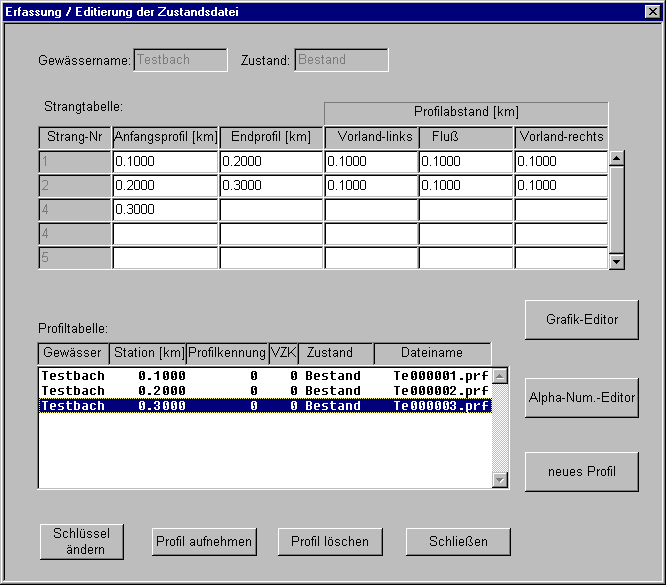
\includegraphics[width=1.0\textwidth]{ErfassungEditierungZustandsdatei}
   \caption{Die Maske zum Erfassen und Editieren der Zustandsdatei}
   \label{Einstieg Abb ErfassungEditierungZustandsdatei}
\end{figure}


\subsection{Ein neues Profil anlegen}
\label{Einstieg Subsec ProfilAnlegen}

Sofern Sie eine neue Zustandsdatei angelegt haben, enth\"{a}lt der Dialog \dialog{Erfas\-sung/Edi\-tierung der Zustandsdatei}
keine Eintr\"{a}ge. Die Strangtabelle im oberen Teil der Dialogmaske und die Profiltabelle im unteren Teil, die automatisch
beim Anlegen eines Profils ausgef\"{u}llt werden, sind leer. In diesem Fall k\"{o}nnen Sie entweder \"{u}ber die Option
\schalter{Profil aufnehmen} bereits existierende Profile (im BCE-Format) in den Zustand \"{u}bernehmen, oder aber ein neues
Profil anlegen. In letzterem Fall w\"{a}hlen Sie die Schaltfl\"{a}che \schalter{Neues Profil}. Es erscheint eine Maske, die Sie
zur Angabe des Profilschl\"{u}ssels auffordert, \"{u}ber den die neue Profildatei referenziert werden soll
(Abbildung~\ref{Einstieg Abb Profilschluessel}).
\begin{figure}[ht]
   \centering
   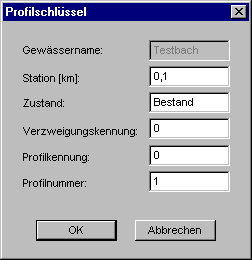
\includegraphics[width=0.4\textwidth]{Profilschluessel}
   \caption{Eingabemaske f\"{u}r den Profilschl\"{u}ssel}
   \label{Einstieg Abb Profilschluessel}
\end{figure}

Der Profilschl\"{u}ssel setzt sich aus dem Gew\"{a}ssernamen (es wird der Name \"{u}bernommen, den Sie der entsprechenden
Zustandsdatei zugeordnet haben), der Stationsangabe (in $\mathrm{km}$), dem Profilzustand (es wird der Zustand der
Verkn\"{u}pfungsdatei vorgeschlagen) sowie der Verzweigungs- und Profilkennung zusammen. Innerhalb eines Projektes darf ein
Profilschl\"{u}ssel nur einmal vorkommen, d.h. es k\"{o}nnen keine Profile mit identischem Gew\"{a}ssernamen, Profilzustand, sowie
der gleichen Verzweigungs- und Profilkennung an einer Station existieren.

Standardm\"{a}{\ss}ig werden Ihnen bei der Verzweigungs- und Profilkennung die Werte $0$ vorgeschlagen (keine Verzweigung,
keine Mehrfeldbr\"{u}cke). Zus\"{a}tzlich k\"{o}nnen sie in dem Feld \dialog{Profilnummer} eine pers\"{o}nliche Identifikation f\"{u}r das
Profil eingeben, die Ihnen z.B. die Zuordnung zum entsprechenden Aufma{\ss} erleichtert. Die Stationierungsrichtung ist
nicht festgelegt. Es wird jedoch empfohlen, im Sinne des Gew\"{a}sserverzeichnisses~NRW grunds\"{a}tzlich von der M\"{u}ndung
($\mathrm{km}~0$) in Richtung Quelle aufsteigend zu stationieren.

Die Profile k�nnen in beliebiger Reihenfolge eingegeben werden. Die Sortierung erfolgt au\-to\-ma\-tisch anhand der Stationierung in aufsteigender Reihenfolge. Soll umgekehrt sta\-tio\-niert wer\-den, ist unter \menu{\marrow Extras \marrow Optionen} bei der Sortierung der Strangtabelle \schalter{r�ckw�rts} zu w�h\-len. Nach der Eingabe des Profilschl�ssels und Best�tigung mit \schalter{OK} gelangen Sie auto\-ma\-tisch in den alpha\-nu\-me\-ri\-schen Editor (Abbildung~\ref{Einstieg Abb AlphanumerischerEditor}).

\subsection{Dateneingabe im alphanumerischen Editor}

Aus dem Dialog \dialog{Erfassung/Editierung der Zustandsdatei} gelangen Sie \"{u}ber die Schaltfl\"{a}che
\schalter{Alpha-Num.-Editor} in den alphanumerischen Editor (Abbildung~\ref{Einstieg Abb AlphanumerischerEditor}). Beim
Anlegen eines neuen Profilschl\"{u}ssels wird dieser automatisch ge\"{o}ffnet. Mit seiner Hilfe lassen sich profilbezogene Daten
eingeben und ver\"{a}ndern.

In der rechten oberen Ecke werden Ihnen die wichtigsten Schl\"{u}sseldaten des Profils, wie z.B. Gew\"{a}ssername und
Stationswert angezeigt. Darunter finden Sie ein Editierfeld, in dem Sie einen Kommentar speziell zu dem aktuellen
Profil eingeben k\"{o}nnen. In der linken Bildh\"{a}lfte befindet sich eine Tabelle, in der die Werte f\"{u}r den jeweils in dem
Listenfeld der rechten Bildh\"{a}lfte (unter dem Kommentar) angezeigten Datensatz eingegeben werden k\"{o}nnen. Wenn Sie noch
keine anderen sogenannten Datenblocktypen (siehe Abschnitt~\ref{Einstieg Subsec Grafikeditor}) angelegt haben,
erscheint beim Klicken auf den Pfeil des Listenfeldes nur die Gel\"{a}ndeh\"{o}he.
\begin{figure}[hbt]
   \centering
   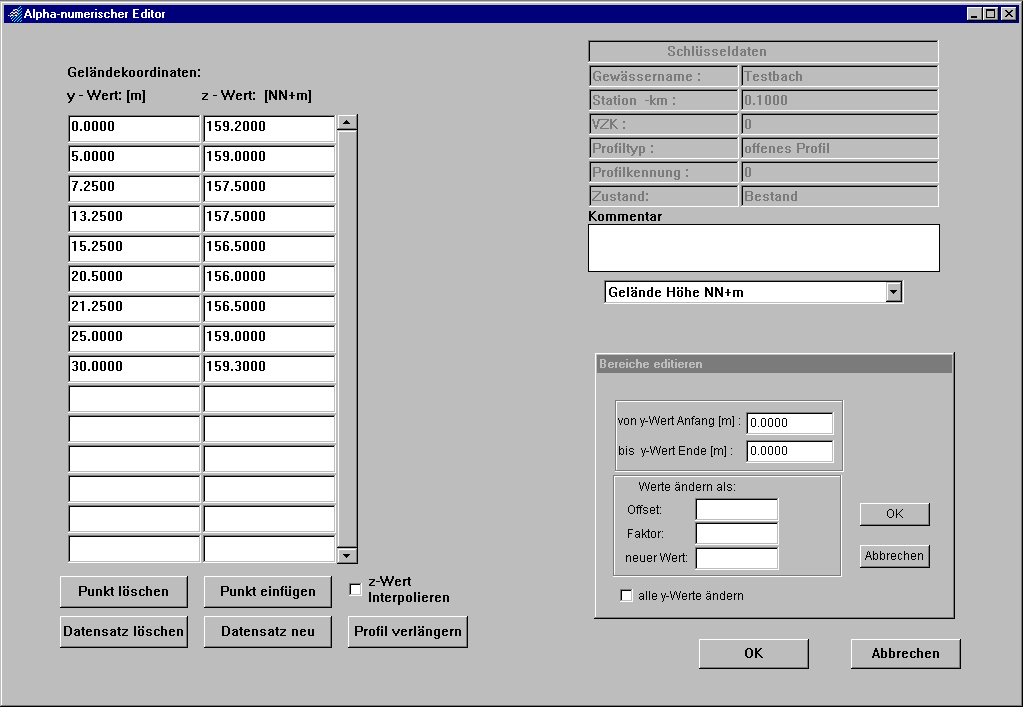
\includegraphics[width=1.0\textwidth]{AlphanumerischerEditor}
   \caption{Der alphanumerische Editor}
   \label{Einstieg Abb AlphanumerischerEditor}
\end{figure}

Bei Aufruf des alphanumerischen Editors wird standardm\"{a}{\ss}ig zun\"{a}chst der Datensatz Gel\"{a}ndeh\"{o}he angezeigt. Die
Gel\"{a}ndeh\"{o}he mu{\ss} in jedem Fall (auch bei Sonderprofilen wie z.B. Durchl\"{a}ssen) eingeben werden und stellt den Bezug f\"{u}r
alle weiteren Datens\"{a}tze dar. Bei dem Datensatz Gel\"{a}ndeh\"{o}he besteht das Spreadsheet aus zwei Spalten f\"{u}r die
Gel\"{a}ndekoordinaten des Profils.

Die $y$-Werte bezeichnen die Distanz der Me{\ss}- bzw. Profilpunkte zu einem Referenzpunkt im Querprofil. Negative Werte sind
m\"{o}glich. Zur Vermeidung von falschen Zuordnungen sollten die Querprofile grunds\"{a}tzlich in Flie{\ss}richtung gesehen
aufgetragen werden. Der allgemein \"{u}blichen Konvention entsprechend erfolgt die Zuordnung von links nach rechts in
Flie{\ss}richtung. Die $z$-Werte geben die Gel\"{a}ndeh\"{o}he in [NN+m] an den jeweiligen Profilpunkten wieder.

Maximal k\"{o}nnen bis zu 500~Profilpunkte in einem Querprofil angelegt werden. Bei \"{a}lteren Versionen des Berechnungsprogramms
kann die Anzahl von Profilpunkten aus Speicherplatzgr\"{u}nden noch auf 50 beschr\"{a}nkt sein. Eine Profildatei besteht aus
mindestens zwei Gel\"{a}ndekoordinaten.
\begin{hinweis}
   Anstelle der Gel\"{a}ndeh\"{o}he in [NN+m] kann auch ein anderes H\"{o}henbezugssystem gew\"{a}hlt werden, z.B.
   [m+HN]. Ist ein Anschlu{\ss} an ein H\"{o}henbezugssystem nicht vorhanden, so w\"{a}hlen Sie sich einen Referenzpunkt und
   weisen ihm eine fiktive H\"{o}henangabe zu.
\end{hinweis}

Die Tabellenwerte im Spreadsheet des alphanumerischen Editors k\"{o}nnen vom Benutzer direkt editiert werden. Indem der
Mauszeiger auf das entsprechende Editierfeld bewegt und ein neuer Wert eingegeben wird, k\"{o}nnen die angezeigten Daten
ge\"{a}ndert bzw. neue Daten eingegeben werden. \"{U}ber die Tabulator- und Entertaste ist ein Springen zwischen den Editierfeldern
m\"{o}glich. Punkt oder Komma machen bei der Dateneingabe keinen Unterschied.

Die $y$- und zugeh\"{o}rigen $z$-Werte werden in der Reihenfolge gespeichert, wie Sie sie im Spreadsheet eingegeben haben.
Bei Normalprofilen ist eine Sortierung der $y$-Werte in aufsteigender Reihenfolge zu gew\"{a}hrleisten. Lediglich bei
Profilen mit R\"{u}ckspr\"{u}ngen kann davon abgewichen werden\footnote{Zur besseren Kontrolle werden Profilpunkte an R�ckspr�ngen und senkrechten W�nden im Textfeld rot markiert.}. \"{U}ber die Schaltfl\"{a}chen \schalter{Punkt einf\"{u}gen} und
\schalter{Punkt l\"{o}schen} wird vor dem Wert, auf dem sich der Cursor befindet, ein Punkt eingef\"{u}gt, bzw. der Wert des
aktuellen Editierfeldes gel\"{o}scht.

Es ist auch m\"{o}glich einen Punkt interpolieren zu lassen. Dazu f\"{u}gen Sie zun\"{a}chst einen Punkt ein, markieren dann die
Checkbox \checkbox{z-Wert interpolieren}, geben den $y$-Wert ein und klicken in das Feld f\"{u}r die $z$-Werte. Es erscheint
die linear interpolierte Gel\"{a}ndeh\"{o}he an der Stelle des $y$-Wertes.
\begin{hinweis}
   Vermeiden Sie die Eingabe von genau vertikalen W\"{a}nden, da sich dort in der Regel auch die Trennfl\"{a}chen befinden. Diese
   werden dann unter Umst\"{a}nden vom Programm nicht eindeutig zugeordnet.
\end{hinweis}

Um neue Datenblocktypen f\"{u}r das Profil anzulegen, w\"{a}hlen Sie den Schalter \schalter{Datensatz neu}. Zu empfehlen ist es,
die Gel\"{a}ndeh\"{o}he im alphanumerischen Editor einzugeben, diesen mit \schalter{OK} (Speichern) zu verlassen und anschlie{\ss}end
in den Grafik\-editor zu wechseln, um dort weitere Datens\"{a}tze anzulegen. Sie k\"{o}nnen aber auch alle Eingaben im
alphanumerischen Editor vornehmen.
\begin{hinweis}
   Kontrollieren Sie die Profilform indem Sie nach der Dateneingabe in den Grafikeditor wechseln.
   Sie beugen damit Tippfehlern als auch Fehler in der Eingabereihenfolge der Punkte vor.
\end{hinweis}
Haben Sie vor dem Verlassen des Editors die Datens\"{a}tze \afz{Rauheit}, \afz{Trennfl\"{a}chen} und \afz{durchstr\"{o}mte Bereiche}
nicht angelegt, so werden Sie vor die Frage gestellt, ob \wspwin{} diese automatisch f\"{u}r Sie erstellen soll. Die
Trennfl\"{a}chen und die Grenzen des durchstr\"{o}mten Bereiches werden bei der automatischen Generierung am \"{a}u{\ss}eren Rand Ihres
Profils eingef\"{u}gt. Die Rauheit kann nur automatisch erstellt werden, wenn zuvor unter dem Men\"{u} \menu{\marrow
E\underline{x}tras \marrow \underline{O}ptionen} eine automatische Generierung der Rauheit vereinbart wurde (siehe hierzu Abschnitt~\ref{Installation Subsec Standardeinstellungen}).


\subsection{Dateneingabe im Grafikeditor}
\label{Einstieg Subsec Grafikeditor}

Neben dem Editieren der Profildateien im alphanumerischen Editor existiert in \wspwin{} auch eine wesentlich einfachere
und anschaulichere M\"{o}glichkeit Eingabewerte zu editieren, n\"{a}mlich der Grafikeditor. Der grafische Editor wird wie der
alphanumerische Editor aus dem Dialogfenster \dialog{Erfassung/Editierung der Zustandsdatei} heraus aufgerufen.

Sobald Sie den grafischen Editor aufgerufen haben, erhalten Sie eine grafische Darstellung der Gel\"{a}ndeh\"{o}he f\"{u}r Ihr zuvor
markiertes Profil. Daneben finden Sie in der linken Bildmitte noch einmal die wichtigsten Schl\"{u}sseldaten ihres Profils und
ein Editierfeld f\"{u}r einen beliebigen Kommentartext, sowie in der rechten oberen Ecke, entsprechend des alphanumerischen
Editors, eine editierbare Tabelle der $y$- und $z$-Werte. Wie beim alphanumerischen Editor k\"{o}nnen Sie auch hier \"{u}ber ein
Listenfeld unterschiedliche Datenblocktypen darstellen lassen und zwar sowohl in der Tabelle wie auch in der Grafik.
Standardm\"{a}{\ss}ig wird zun\"{a}chst nur die Gel\"{a}ndeh\"{o}he angezeigt.

Der grafisch-interaktive Editor setzt sich dementsprechend aus einem alphanumerischen Editor und einem grafischen Editor
zusammen, wobei \"{A}nderungen in einem der beiden Editoren eine direkte Aktualisierung des jeweils anderen Editors zur Folge
haben. Sobald Sie einen Zahlenwert im alphanumerischen Editor \"{a}ndern und das Editierfeld verlassen, wird die Grafik
aktualisiert und Sie k\"{o}nnen das Resultat anschaulich bewerten. Umgekehrt k\"{o}nnen Sie direkt in der Grafik f\"{u}r jeden
Profilpunkt, der durch eine senkrechte Linie gekennzeichnet ist, \"{A}nderungen vornehmen.
\begin{figure}
   \centering
   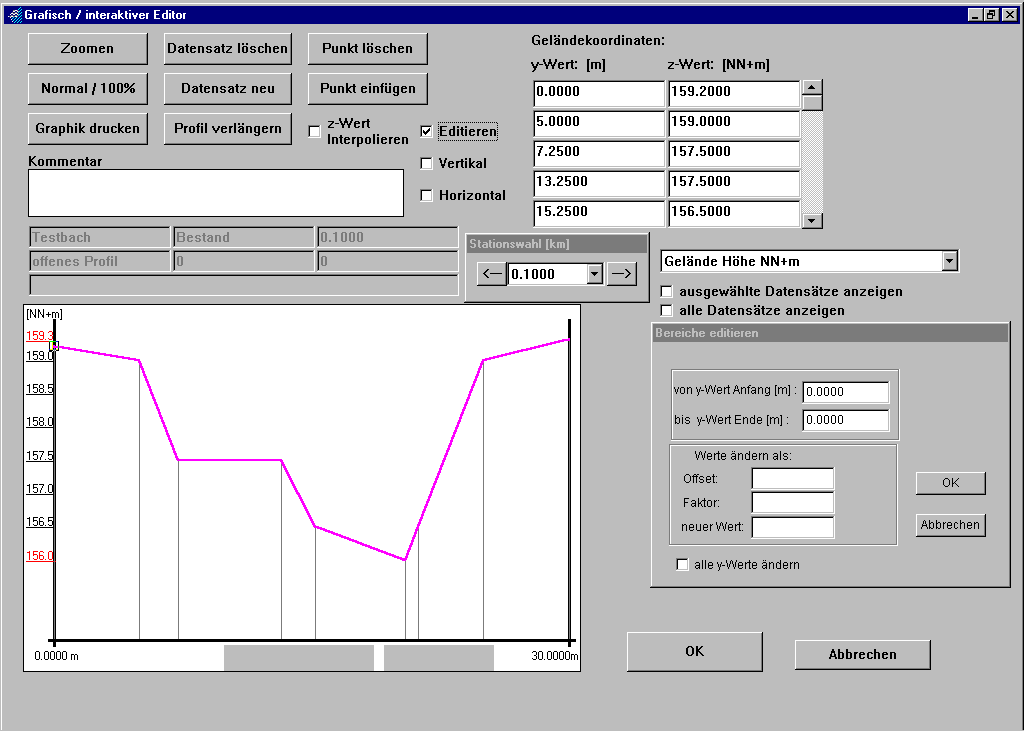
\includegraphics[width=1.0\textwidth]{Grafikeditor}
   \caption{Der Grafikeditor}
   \label{Einstieg Abb Grafikeditor}
\end{figure}

Sobald Sie die Maus in die Grafik bewegen, wandelt sich der Mauszeiger in ein Fadenkreuz um. Unter der Grafik erscheinen
die $y$- und $z$-Koordinaten f\"{u}r den Punkt, an dem sich das Fadenkreuz gerade befindet. Ein K\"{a}stchen \"{u}ber dem Profilpunkt
in der Grafik zeigt Ihnen gleichzeitig Ihre aktuelle Position im alphanumerischen Editor. Sobald Sie sich im
alphanumerischen Editor bewegen, wandert auch das K\"{a}stchen. Damit behalten Sie den \"{U}berblick \"{u}ber beide Editoren und
k\"{o}nnen Ver\"{a}nderungen im jeweils anderen Editor unmittelbar wahrnehmen. Die Schaltfl\"{a}chen \schalter{Punkt einf\"{u}gen},
\schalter{Punkt l\"{o}schen}, \schalter{Datensatz neu}, \schalter{Datensatz l\"{o}schen} sowie \schalter{Profil verl\"{a}ngern}
entsprechen denen des alphanumerischen Editors. Daneben finden Sie ganz links die Funktionen \schalter{Zoomen},
\schalter{Normal/100\%} und \schalter{Grafik drucken}.

Um einen Ausschnitt des Profils vergr\"{o}{\ss}ert darzustellen w\"{a}hlen sie \schalter{Zoomen} und markieren mit gedr\"{u}ckter linker
Maustaste den Grafikausschnitt, den sie vergr\"{o}{\ss}ert betrachten m\"{o}chten. Mit \schalter{Normal/100\%} stellen Sie den
urspr\"{u}nglichen Zustand wieder her. Neben der Gel\"{a}ndeh\"{o}he sind weitere Datenblocktypen in \wspwin{} verf\"{u}gbar.
Tabelle~\ref{Einstieg Tab GrafischeDatenblocktypen} gibt einen \"{U}berblick, welche Datenblocktypen grafisch dargestellt und
welche zus\"{a}tzlich grafisch-interaktiv bearbeitet werden k\"{o}nnen. Um sich mehrere Datenblocktypen in der Grafik anzeigen zu
lassen markieren Sie die Option \checkbox{ausgew\"{a}hlte Datens\"{a}tze anzeigen} und w\"{a}hlen daraufhin die gew\"{u}nschten Datens\"{a}tze
aus dem Listenfeld aus. Die Option \checkbox{alle Datens\"{a}tze anzeigen} f\"{u}gt alle darstellbaren Datenbl\"{o}cke in die Grafik
ein.
\begin{table}
   \centering
   \input{Einstieg/tab/Datenblocktypen.tab}
   \caption{Grafische Bearbeitung der Datenblocktypen}
   \label{Einstieg Tab GrafischeDatenblocktypen}
\end{table}

\"{A}nderungen der Gel\"{a}ndeh\"{o}he k\"{o}nnen in der Grafik schnell und unkompliziert dadurch vorgenommen werden, da{\ss} Sie sich,
nachdem Sie die Kontrollk\"{a}stchen \checkbox{Editieren} und \checkbox{Horizontal} oder \checkbox{Vertikal} aktiviert haben,
mit der Maus an den gew\"{u}nschten Profilpunkt bewegen und bei gedr\"{u}ckter linker Maustaste die Gel\"{a}ndekontur verziehen. Der
alphanumerische Editor wird sodann aktualisiert. Beachten Sie, da{\ss} die grafische Darstellung grunds\"{a}tzlich an den h\"{o}chsten
und niedrigsten Gel\"{a}ndeh\"{o}hen orientiert ist, was zu einer starken \"{U}berh\"{o}hung und nicht ma{\ss}st\"{a}blichen Darstellungen f\"{u}hrt.
Zwischen einzelnen Profilen k\"{o}nnen Sie ohne den Grafik-Editor zu verlassen durch Klicken der Pfeiltasten auf dem
Listenfeld \dialog{Stationswahl} und Auswahl des entsprechenden Profils springen.


\subsection{Bereiche editieren}
\label{Einstieg Subsec BereicheEditieren}

Eine weitere Hilfe f\"{u}r die Dateneingabe der Gel\"{a}ndeh\"{o}hen im alphanumerischen und im grafischen Editor bietet der Dialog
\dialog{Bereiche editieren}. Hier k\"{o}nnen mehrere Werte gleichzeitig ge\"{a}ndert werden. Besonders vorteilhaft ist dies bei
regelm\"{a}{\ss}igen Gerinnen in denen sich nur die Gel\"{a}ndeh\"{o}he \"{a}ndert.
\begin{figure}[hbt]
   \centering
   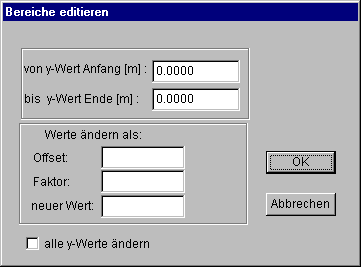
\includegraphics[width=0.5\textwidth]{BereicheEditieren}
   \caption{Dialogfenster zum Editieren von Bereichen}
   \label{Einstieg Abb BereicheEditieren}
\end{figure}

Legen Sie dazu zun\"{a}chst den zu editierenden Bereich mit Hilfe der Felder $y$-Wert Anfang und Ende fest oder aktivieren Sie
das Kontrollfeld \checkbox{alle y-Werte \"{a}ndern}. Im Grafikeditor kann der zu \"{a}ndernde Bereich auch durch verschieben der
Maus \"{u}ber der Grafik bei gedr\"{u}ckter linker Maustaste festgelegt werden. Die Felder Offset, Faktor und neuer Wert bewirken
folgendes:
\begin{description}
   \item[Offset:]
      Der hier eingegebene Wert wird zu den Gel\"{a}ndeh\"{o}hen des ausgew\"{a}hlten Bereiches abh\"{a}ngig vom Vorzeichen addiert oder
      subtrahiert.
   \item[Faktor:]
      Es erfolgt eine Multiplikation aller Gel\"{a}ndeh\"{o}hen im ausgew\"{a}hlten Bereich mit dem angegebenen Wert.
   \item[Neuer Wert:]
      Alle Gel\"{a}ndeh\"{o}hen des ausgew\"{a}hlten Bereichs werden auf den hier eingegebenen Zahlenwert ge\"{a}ndert.
\end{description}
Bitte beachten Sie, da{\ss} die Funktionen nur einzeln ausgef\"{u}hrt werden k\"{o}nnen.


\subsection{Neue Datens\"{a}tze anlegen}

Mit dem Schalter \schalter{Datensatz neu} aus dem alphanumerischen oder Grafikeditor heraus haben Sie die M\"{o}glichkeit,
neben der Gel\"{a}ndeh\"{o}he auch andere Datenblocktypen in das Profil aufzunehmen. Ein Normalprofil besteht immer mindestens
aus den Datens\"{a}tzen
\begin{itemize}
   \item Gel\"{a}ndeh\"{o}he
   \item Rauheit
   \item Trennfl\"{a}chen
   \item Durchstr\"{o}mte Bereiche
\end{itemize}
die mit Hilfe von \wspwin{} beim Verlassen des Editors auch automatisch generiert werden k\"{o}nnen.

Beim Neuanlegen eines Datensatzes erscheint zun\"{a}chst wiederum ein Listenfeld, aus dem Sie einen Datenblock w\"{a}hlen k\"{o}nnen.
Anschlie{\ss}end sind Werte (in Abh\"{a}ngigkeit vom Typ) zum neu eingef\"{u}gten Datenblock einzugeben. Eine \"{U}bersicht \"{u}ber die
vorhandenen Datensatztypen gibt Tabelle~\ref{Einstieg Tab GrafischeDatenblocktypen} in Abschnitt~\ref{Einstieg Subsec
Grafikeditor}.

Ein Datensatz kann inklusive seiner Werte \"{u}ber den Schalter \schalter{Datensatz l\"{o}schen} wieder aus der Profildatei
entfernt werden. Die Dateneingabe f\"{u}r die einzelnen Datens\"{a}tze sind in den nachfolgenden Kapiteln n\"{a}her erl\"{a}utert.


\subsection{Rauheit eingeben}
\label{Einstieg Subsec Rauheit}

Rauheiten k\"{o}nnen in \wspwin{} wahlweise als \autor{Darcy-Weisbach}-Rauheiten ($k_S$-Werte in [$\mathrm{m}$]) oder
\autor{Manning-Strickler}-Rauheiten ($k_{ST}$-Werte in [$\mathrm{m^{1/3}/s}$]) eingegeben werden. Sobald Sie \"{u}ber den
Schalter \schalter{Datensatz neu} den Datenblocktyp Rauheit eingef\"{u}gt haben (entweder als $k_S$- oder $k_{ST}$-Werte --
die Datens\"{a}tze schlie{\ss}en sich gegenseitig aus), \"{o}ffnet sich im Spreadsheet des alphanumerischen oder grafischen Editors
neben den $y$-und $z$-Werten der Gel\"{a}ndeh\"{o}he eine 3.~Spalte, in der Sie den einzelnen Profilpunkten Rauheiten zuordnen
k\"{o}nnen.
\begin{hinweis}
   Beachten Sie bei der Festlegung des Datenblocktyps f\"{u}r die Rauheit, da{\ss} dieser die Grundlage f\"{u}r die Auswahl der
   Berechnungsmethode darstellt. Es ist z.B. nicht m\"{o}glich die Berechnung nach dem Flie{\ss}gesetz von \autor{Manning-Strickler}
   auf Basis der \autor{Darcy-Weisbach}'schen Rauheiten durchzuf\"{u}hren.
\end{hinweis}

Haben Sie den Datensatz Rauheit eben erst neu angelegt, brauchen nur die Profilpunkte besetzt werden, an denen eine
\"{A}nderung der Rauheit gegen\"{u}ber den vorherigen Profilpunkten stattfindet. Alle nachfolgenden Profilpunkte werden beim
Speichern der Datei \"{u}ber \schalter{OK} mit dem jeweils davor besetzten Wert aufgef\"{u}llt. Sind die Rauheiten im
Spread\-sheet bereits durch den Wert $0,00$ vorbelegt (z.B. bei einer automatischen Generierung der Rauheiten nach
Abschnitt~\ref{Installation Subsec Standardeinstellungen}), so m\"{u}ssen sie alle Werte neu angeben.

Neben der alphanumerischen Eingabe k\"{o}nnen die Rauheiten auch grafisch-interaktiv ver\"{a}ndert werden. W\"{a}hlen Sie
dazu zun\"{a}chst den Datenblocktyp Rauheit aus dem Listenfeld. Markieren Sie nun mit gedr\"{u}ckter linker Maustaste den
Bereich in der Grafik, den Sie ver\"{a}ndern m\"{o}chten. Es erscheint ein Dialogfenster mit dem Sie wiederum Bereiche im
Querprofil anpassen k\"{o}nnen. Zus\"{a}tzlich zu den in Abschnitt~\ref{Einstieg Subsec BereicheEditieren} angegebenen
Funktionen enth\"{a}lt der Dialog eine Schaltfl\"{a}che \schalter{Datenbank}. Der Umgang mit der Rauheitsdatenbank wird in
Abschnitt~\ref{Fortgeschrittene Subsec Rauheitsdatenbank} n\"{a}her erl\"{a}utert.

Beachten Sie, dass eine Ver�nderung der Trennfl�chen eine �nderung der Rauheitswerte nach sich ziehen kann 	(siehe Abschnitt~\ref{sec:einstieg:profildaten:trennflaechen}).

\begin{table}[hbtp]
   \centering
   \input{Einstieg/tab/Einzelrauheiten.tab}
   \caption{Typische Einzelrauheiten}
   \label{Einstieg Tab Einzelrauheiten}
\end{table}

\subsection{Trennfl\"{a}chen definieren}
\label{sec:einstieg:profildaten:trennflaechen}

Die verwendeten Bestimmungsgleichungen f\"{u}r die Querschnittswerte und die hydraulischen Kenngr\"{o}{\ss}en sind auf dreifach
gegliederte Querschnitte (Abbildung~\ref{Einstieg Abb Teilabflussflaechen}) abgestimmt (linkes Vorland, Flu{\ss}schlauch,
rechtes Vorland). Die Teilabflu{\ss}fl\"{a}chen werden als Stromr\"{o}hren mit horizontalem Wasserspiegel gleicher H\"{o}he aufgefa{\ss}t.
\begin{figure}[hbt]
   \begin{minipage}{1.0\textwidth}
      \centering
      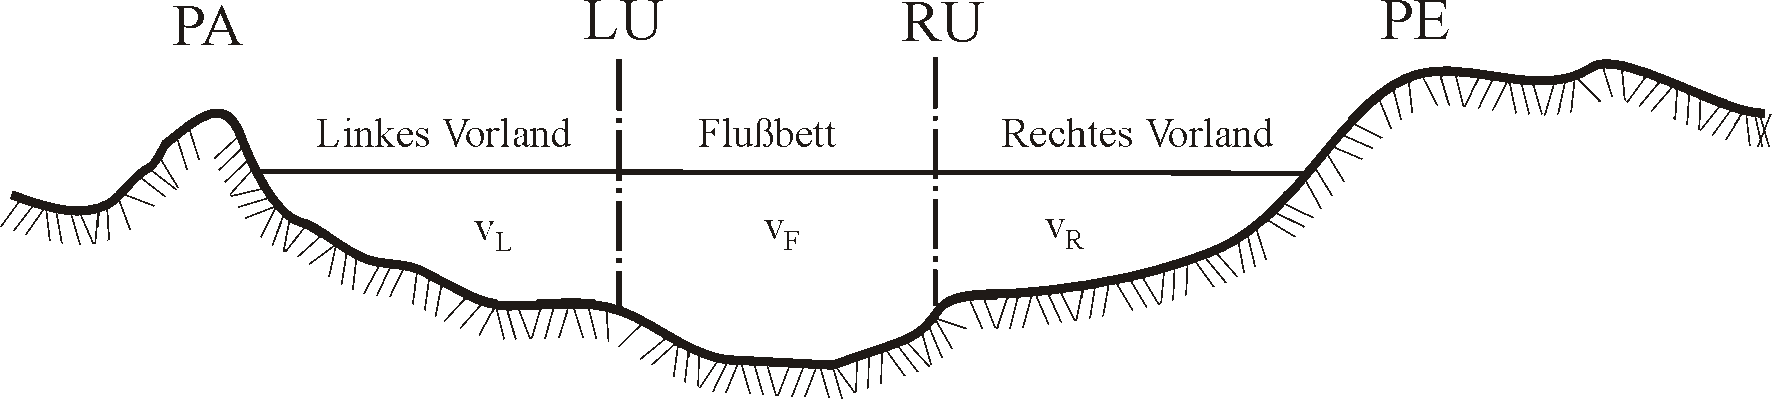
\includegraphics[width=1.0\textwidth]{Trennflaechen}
      \caption{Teilabflu{\ss}fl\"{a}chen eines Flie{\ss}querschnitts}
      \label{Einstieg Abb Teilabflussflaechen}
      \vspace{12pt}
   \end{minipage}
   \begin{minipage}{1.0\textwidth}
      \centering
      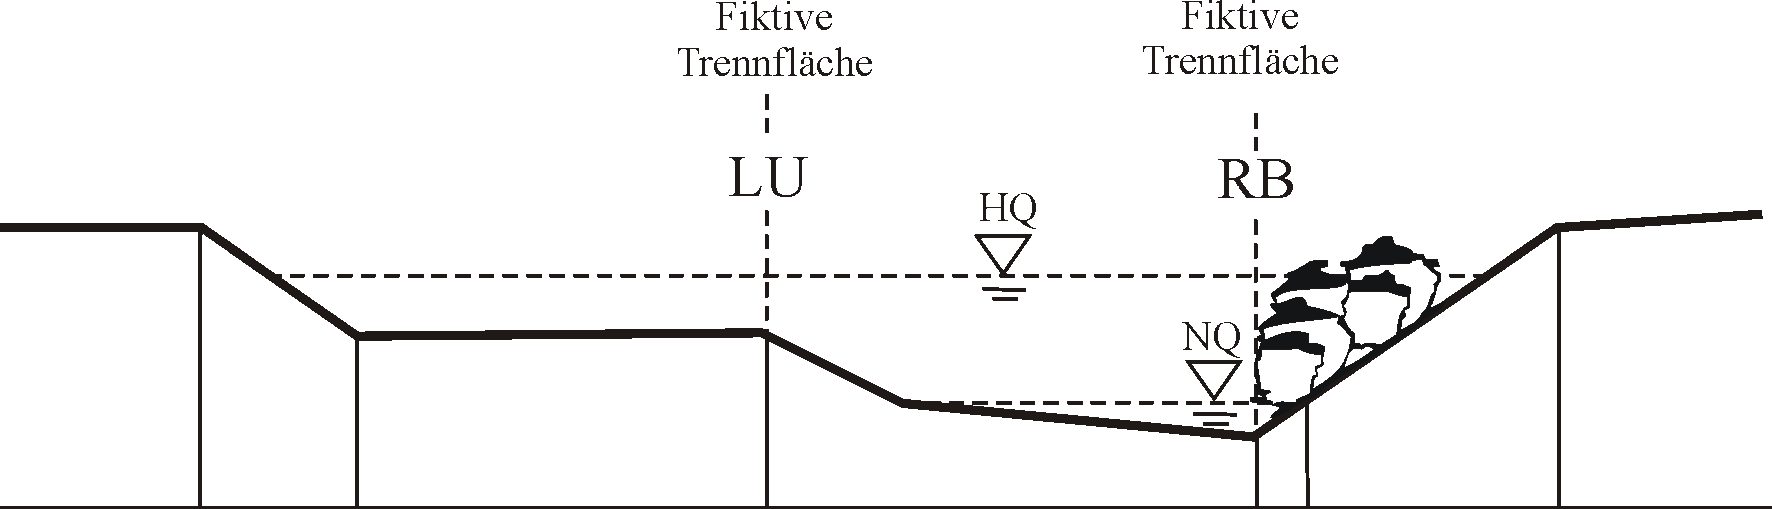
\includegraphics[width=1.0\textwidth]{TrennflaechenBewuchs}
      \caption{Lage der Trennfl\"{a}che bei B\"{o}schungsbewuchs}
      \label{Einstieg Abb Boeschungsbewuchs}
   \end{minipage}
\end{figure}
Die Gliederung des Querschnitts in Teilabflu{\ss}fl\"{a}chen wird durch die Definition der Lage fiktiver Trennfl\"{a}chen festgelegt.
\begin{quote}
   \begin{labeling}[:]{RU (Rechtes Ufer)}
      \item[PA (Profilanfang)]  Anfang des abflu{\ss}wirksamen Querschnitts \newline (linke Grenze des durchstr\"{o}mten Bereichs)
      \item[LU (Linkes Ufer) ]  Grenzpunkt zwischen linkem Vorland und Flu{\ss}schlauch (linke Trennfl\"{a}che)
      \item[RU (Rechtes Ufer)]  Grenzpunkt zwischen Flu{\ss}schlauch und rechtem Vorland (rechte Trennfl\"{a}che)
      \item[PE (Profilende)  ]  Ende des abflu{\ss}wirksamen Querschnitts \newline (rechte Grenze des durchstr\"{o}mten Bereichs)
   \end{labeling}
\end{quote}
Bei Profilen mit Bewuchs ist zu beachten, da{\ss} bei bepflanzten B\"{o}schungen jeweils der B\"{o}schungsfu{\ss}punkt als Grenzpunkt
zwischen Flu{\ss}schlauch und Vorland zu definieren ist (Abbildung~\ref{Einstieg Abb Boeschungsbewuchs}).
\begin{figure}[hbt]
   \centering
   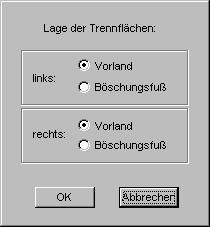
\includegraphics[width=0.35\textwidth]{LageTrennflaechen}
   \caption{Festlegen der Lage der Trennfl\"{a}chen}
   \label{Einstieg Abb LageTrennflaechen}
\end{figure}

Nachdem Sie einen neuen Datensatz \afz{Trennfl\"{a}chen} \"{u}ber den Schalter \schalter{Datensatz neu} angelegt haben, erscheint
ein Sonderdialog, in dem zun\"{a}chst als linker und rechter Profilpunkt f\"{u}r die Trennfl\"{a}chen die beiden \"{a}u{\ss}ersten
Profilpunkte angegeben sind. Diese Werte k\"{o}nnen Sie, je nachdem wo die Trennfl\"{a}chen positioniert werden sollen, mit
anderen $y$-Werten \"{u}berschreiben. Auch beim automatischen Anlegen der Trennfl\"{a}chen werden diese immer nach au{\ss}en gesetzt.

Per Voreinstellung markieren die Trennfl\"{a}chen den \"{U}bergang von der B\"{o}schung auf das Vorland. \"{U}ber den Schalter
\schalter{Lage...} haben Sie aber auch die M\"{o}glichkeit die Lage bei Bewuchs (Abbildung~\ref{Einstieg Abb
Boeschungsbewuchs}) rechts oder links an den B\"{o}schungsfu{\ss} zu legen.
\begin{figure}[hbt]
   \centering
   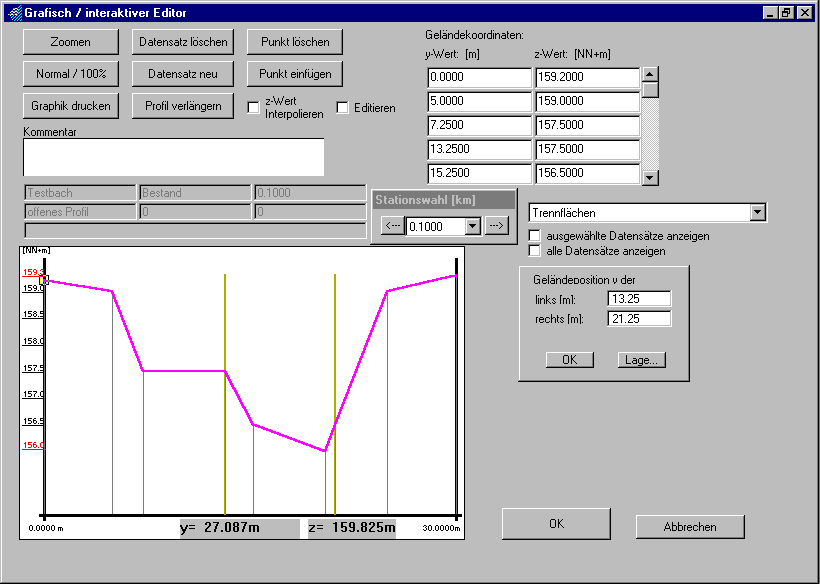
\includegraphics[width=1.0\textwidth]{PositionierungTrennflaechen}
   \caption{Positionierung der Trennfl\"{a}chen}
   \label{Einstieg Abb PositionierungTrennflaechen}
\end{figure}

Sobald Sie Werte eingegeben haben, erscheinen die Trennfl\"{a}chen in der Grafik als gelbe senkrechte Linien. Die gelben Linien k\"{o}nnen in der grafischen Darstellung bei gedr\"{u}ckter linker Maustaste an die gew\"{u}nschte Position im Querprofil verschoben werden. Parallel dazu  werden die entsprechenden aktualisierten Werte im Sonderdialog angezeigt. Wenn Sie den Sonderdialog geschlossen haben, k\"{o}nnen Sie diesen jederzeit durch Klick in der Grafik oder auf das Listenfeld wieder aktivieren. 

Wurde, wie im vorhergehenden Abschnitt beschrieben, bereits ein Datensatz Rauheiten angelegt, so bewirkt jedes Ver�ndern der Trennfl�chen eine automatische Anpassung der Rauheiten, sofern sich allen drei Fliesszonen (links Vorland, Haupt�ffnung und rechtes Vorland) ein eindeutiger Rauheitswert zuordnen l�sst. Ist letzteres nicht der Fall, d.h. wenn innerhalb einer Fliesszone verschiedene Rauheitswerte definiert sind, werden die Rauheiten beibehalten.

Die Position der Trennfl\"{a}chen sollte in jedem Fall festgelegt werden, auch wenn es sich um einen einteiligen
Querschnitt handelt (die Trennfl\"{a}chen w\"{a}ren dann nach au{\ss}en zu legen), da sich andere Programmfunktionen (z.B.
Interpolation, Rauheiten global \"{a}ndern) an den Trennfl\"{a}chen orientieren.




\subsection{Durchstr\"{o}mte Bereiche festlegen}

Neben der Lage der Trennfl\"{a}chen sind in jedem Fall auch stets die linke und rechte Grenze des abflu{\ss}wirksamen Querschnitts
einzugeben. Das hei{\ss}t Totwasserzonen bzw. nicht am Abflu{\ss}geschehen beteiligte Bereiche sind abzugrenzen. Die
Verbindungslinie der Abflu{\ss}-Grenzpunkte ist dar\"{u}ber hinaus im Lageplan einzutragen. Nur die gleichzeitige Betrachtung von
Querprofil und Lageplan kann hier zu einer nachvollziehbaren Festlegung f\"{u}hren. Eine willk\"{u}rliche Verschiebung der
Grenzpunkte allein im Querprofil ist unzul\"{a}ssig.

Die Dateneingabe erfolgt \"{a}hnlich wie bei der Festlegung der Lage der Trennfl\"{a}chen. Allerdings sind in dem hier
erscheinenden Sonderdialog links und rechts sowohl $y$- wie auch $z$-Werte einzugeben. Die Plausibilit\"{a}t wird \"{u}berpr\"{u}ft.
Die Darstellung in der Grafik erfolgt durch senkrechte blaue Linien, die am oberen Bildrand unabh\"{a}ngig von der H\"{o}he der
Werte miteinander verbunden und bei gedr\"{u}ckter linker Maustaste verschiebbar sind.
\begin{figure}[hpbt]
   \centering
   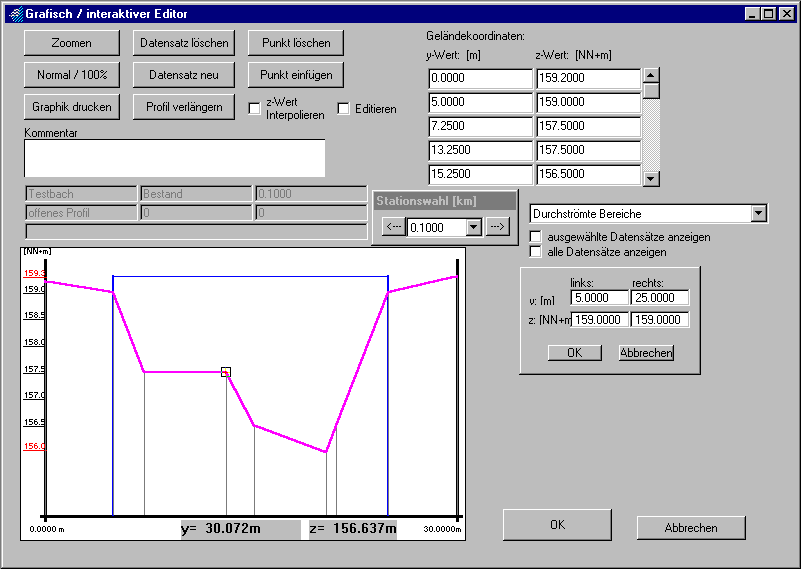
\includegraphics[width=1.0\textwidth]{DurchstroemteBereiche}
   \caption{Abgrenzung der durchstr\"{o}mten Bereiche von Totwasserzonen}
   \label{Einstieg Abb Totwasserzonen}
\end{figure}


\subsection{Georeferenzierung}

Um �berschwemmungsgebiete auszuweisen und zu visualisieren, bzw. auch um mit \wspwin{}-Mapper arbeiten zu k�nnen, m�ssen f�r jedes Profil und jeden Profilpunkt Gauss-Kr�ger-Koordinaten vorliegen. Hierzu m�ssen zun�chst die Datens�tze ''Rechtswert'' und ''Hochwert'' neu angelegt werden. In der Regel ist es ausreichend, wenn f�r den Anfangs- und Endpunkt Koordinaten eingef�gt werden. �ber das Interpolationssymbol rechts neben dem Listknopf k�nnen die fehlenden Werte automatisch zwischen geschaltet werden.
 
\begin{figure}[hpbt]
   \centering
   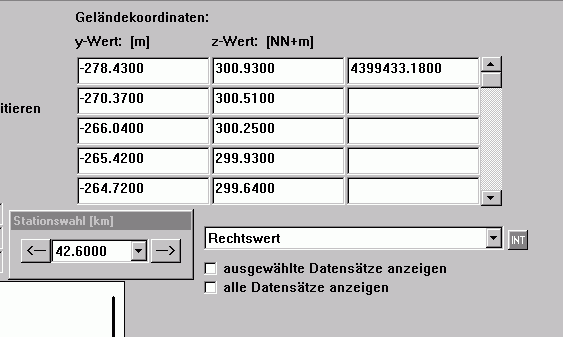
\includegraphics[width=1.0\textwidth]{gauss_krueger}
   \caption{Interpolation fehlender Gauss-Kr�ger-Koordinaten}
   \label{Einstieg Abb Interpolation}
\end{figure}


\subsection{Beispiel Profilbearbeitung}

Erzeugen sie jetzt f\"{u}r den Zustand \afz{Bestand} (siehe Abschnitt~\ref{Einstieg Subsec BeispielZustandsdatei}) drei
Profile im Abstand von jeweils $0,10\unit{km}$.

\subsubsection{Profilschl\"{u}ssel anlegen}
\"{U}ber die Schaltfl\"{a}che \schalter{Neues Profil} in der Maske \dialog{Erfassung/Editierung der Zustandsdatei} gelangen Sie in
den Profilschl\"{u}ssel-Dialog. Geben Sie hier folgendes ein:
\begin{quote}
   \begin{tabular}{ll}
      Gew\"{a}ssername:    &  \beisp{Testbach} \\
      Station:             &  \beisp{0,1} \\
      Zustand:             &  \beisp{Bestand} \\
      Verzweigungskennung: &  \beisp{0} \\
      Profilkennung:       &  \beisp{0} \\
      Profilnummer:        &  \beisp{1} \\
   \end{tabular}
\end{quote}
Mit \schalter{OK} gelangen Sie automatisch in den alphanumerischen Editor.

\subsubsection{Gel\"{a}ndeh\"{o}he eingeben}
Im alphanumerischen Editor finden Sie nun eine Tabelle, in die die folgenden Gel\"{a}ndekoordinaten eingegeben werden m\"{u}ssen.
\begin{quote}
   \begin{tabular}{ccccc}
      $y$-Wert $\mathrm{[m]}$ & $z$-Wert $\mathrm{[NN\!+\!m]}$ & \hspace{1cm} &
      $y$-Wert $\mathrm{[m]}$ & $z$-Wert $\mathrm{[NN\!+\!m]}$ \\[6pt]
      \beisp{~0,00}  & \beisp{159,20}  &  & \beisp{20,50} & \beisp{156,00} \\
      \beisp{~5,00}  & \beisp{159,00}  &  & \beisp{21,25} & \beisp{156,50} \\
      \beisp{~7,25}  & \beisp{157,50}  &  & \beisp{25,00} & \beisp{159,00} \\
      \beisp{13,25}  & \beisp{157,50}  &  & \beisp{30,00} & \beisp{159,30} \\
      \beisp{15,25}  & \beisp{156,50}
   \end{tabular}
\end{quote}

Speichern Sie nun die Eingabe indem sie mit \schalter{OK} den Editor verlassen. Sie erhalten eine Meldung, da{\ss} mindestens
Gel\"{a}ndeh\"{o}he, Trennfl\"{a}chen, durchstr\"{o}mte Bereiche und Rauheiten angegeben werden m\"{u}ssen und Sie werden gefragt, ob
\wspwin{} diese Datens\"{a}tze automatisch anlegen soll. Best\"{a}tigen Sie die automatische Generierung. Haben Sie im Vorfeld
keine Festlegung zur automatischen Generierung der Rauheiten getroffen (vgl. Abschnitt~\ref{Installation Subsec
Standardeinstellungen}), so erhalten Sie die Meldung, da{\ss} der Datensatz \afz{Rauheit} noch nicht erstellt wurde.

In der Profiltabelle erscheint nun Ihre neu angelegte Profildatei. Markieren Sie diese und wechseln Sie in den
grafisch-interaktiven Editor.

\subsubsection{Rauheiten festlegen}
Legen Sie nun f\"{u}r das Profil die Rauheiten an. Wenn Sie unter \menu{\marrow E\underline{x}tras \marrow
\underline{O}ptionen} eine automatische Generierung (Abschnitt~\ref{Installation Subsec Standardeinstellungen}) aktiviert
haben, wurde der Datensatz Rauheit (je nach Einstellung $k_S$- oder $k_{ST}$-Wert) bereits angelegt und die Werte mit null
vorbesetzt. Falls nicht, m\"{u}ssen Sie zun\"{a}chst einen neuen Datensatz erstellen. Mit \schalter{Datensatz neu} \"{o}ffnet sich
eine Auswahlliste, aus der Sie bitte \afz{Rauheit-ks} ausw\"{a}hlen.

Wurden bei der automatischen Generierung \autor{Manning-Strickler}-Rauheiten angelegt, so m\"{u}ssen Sie zun\"{a}chst diesen
Datensatz l\"{o}schen und k\"{o}nnen erst im Anschlu{\ss} daran den Datensatz \afz{Rauheit-ks} erstellen. Bei einer automatischen
Generierung des Rauheitsdatensatzes nach \autor{Darcy-Weisbach} sind diese Ma{\ss}nahmen nicht erforderlich.

In der Eingabemaske rechts oben erscheint jetzt eine zus\"{a}tzliche Spalte mit der Bezeichnung \afz{Rauheit~ks~[m]}. Geben
Sie hier die folgenden Werte ein:
\begin{quote}
   \begin{tabular}{ccccc}
      $\mathbf{y}$-\textbf{Wert} $\mathbf{\mathrm[m]}$   & $\mathbf{k_S~\mathrm{[m]}}$ & \qquad &
      $\mathbf{y}$-\textbf{Wert} $\mathbf{\mathrm[m]}$   & $\mathbf{k_S~\mathrm{[m]}}$ \\[6pt]
      \beisp{~0,00}  &  \beisp{0,20}   && \beisp{20,50} &   \beisp{0,03} \\
      \beisp{~5,00}  &  \beisp{0,20}   && \beisp{21,25} &   \beisp{0,02} \\
      \beisp{~7,25}  &  \beisp{0,05}   && \beisp{25,00} &   \beisp{0,02} \\
      \beisp{13,25}  &  \beisp{0,03}   && \beisp{30,00} &   \beisp{0,02} \\
      \beisp{15,25}  &  \beisp{0,03}
   \end{tabular}
\end{quote}
Ist die Spalte f\"{u}r die Rauheiten im Spreadsheet leer, so werden die Zwischenwerte von \wspwin{} automatisch aufgef\"{u}llt.
Sind jedoch die Rauheiten mit $0,00$ vorbelegt (z.B. durch zwischenzeitliches Speichern der Profildaten), so m\"{u}ssen Sie
auch die Zwischenwerte \"{u}berschreiben.

Markieren Sie dazu beispielsweise in der Grafik den Bereich $0,00\unit{m}$ bis $7,25\unit{m}$ mit gedr\"{u}ckter Maustaste. In
dem Dialog \dialog{Bereiche editieren} wird der markierte Bereich angezeigt. Geben Sie die Rauheit f\"{u}r diesen Bereich in
das Feld
\begin{quote}
   neuer Wert: \quad \beisp{0,2}
\end{quote}
ein und best\"{a}tigen Sie mit \schalter{OK}. In gleicher Weise verfahren Sie mit den \"{u}brigen Bereichen. Um die Werte zu
speichern, verlassen Sie den Editor mit \schalter{OK}.

\subsubsection{Definition der Trennfl\"{a}chen}
Im n\"{a}chsten Schritt erfolgt die Festlegung der Trennfl\"{a}chen. Sofern nicht automatisch generiert, legen Sie mit
\schalter{Datensatz neu} zun\"{a}chst den Datensatz \afz{Trennfl\"{a}chen} an. Der Sonderdialog \dialog{Trennfl\"{a}chen} zeigt Ihnen
nun zun\"{a}chst die Lage der Trennfl\"{a}chen am Rand Ihres Profils.

Verschieben Sie die linke Trennfl\"{a}che (gelbe Linie) mit gedr\"{u}ckter linker Maustaste an die Position $13,25\mathrm{m}$.
Verfahren Sie analog mit der rechten Trennfl\"{a}che bis zur Position $21,25\mathrm{m}$. \"{O}ffnen Sie mit \schalter{Lage...}
den Dialog zur Lagebeschreibung der Trennfl\"{a}che und \"{a}ndern sie diese auf der rechten Profilseite in \afz{B\"{o}schungsfu{\ss}}.
Best\"{a}tigen Sie die Eingabe der Lagebeschreibung und der Trennfl\"{a}chen mit \schalter{OK}.

\subsubsection{Beschr\"{a}nkung des durchstr\"{o}mten Bereichs}
Analog zur Festlegung der Trennfl\"{a}chen erfolgt die Abgrenzung der Totwasserbereiche. Legen Sie dazu ggf. den Datensatz
\afz{Durchstr\"{o}mte Bereiche} neu an. Der Sonderdialog enth\"{a}lt folgende Angaben:
\begin{quote}
   \begin{tabular}{lrr}
      links:   &  $y =\:\:0,00\unit{m}$    &  $z = 159,20\unit{NN\!+\!m}$  \\
      rechts:  &  $y = 30,00\unit{m}$      &  $z = 159,30\unit{NN\!+\!m}$
   \end{tabular}
\end{quote}
Verschieben Sie nun wieder mit der Maus die blaue Begrenzungslinie auf
\begin{quote}
   \begin{tabular}{lrr}
      links:   &  $y =\:\:5,00\unit{m}$    &  $z = 159,00\unit{NN\!+\!m}$  \\
      rechts:  &  $y = 25,00\unit{m}$      &  $z = 159,00\unit{NN\!+\!m}$
   \end{tabular}
\end{quote}
Best\"{a}tigen Sie die Eingabe mit \schalter{OK}.

\subsubsection{Profil kopieren}
Sie k\"{o}nnen nun, um weitere Profile zu erstellen, die Eingabe f\"{u}r die nachfolgenden Profile ebenfalls von Hand vornehmen.
Mit der Funktion \schalter{Profil aufnehmen} aus der Maske \dialog{Erfassung/Editierung der Zustandsdatei} kann aber auch
eine komplette Kopie des Profils erstellt werden. Sie m\"{u}ssen dann lediglich den Profilschl\"{u}ssel \"{a}ndern.

Mit dem Schalter \schalter{Profil aufnehmen} gelangen sie in einen  Dateiauswahldialog. Markieren Sie hier Ihre eben
erstellte Profildatei. Die Frage, ob das Profil kopiert werden soll, beantworten Sie mit \schalter{ja} und gelangen so in
das Dialogfenster zur Eingabe des Profilschl\"{u}ssels. \"{A}ndern sie die Werte
\begin{quote}
   \begin{tabular}{ll}
      Station:       &  \beisp{0,2} \\
      Profilnummer:  &  \beisp{2}
   \end{tabular}
\end{quote}
Das kopierte Profil erscheint in der Profiltabelle. Wiederholen Sie diesen Vorgang zur Erstellung des Querprofils~3,
mit der Station $0,3\unit{km}$.

\subsubsection{Bereiche editieren}
Die Profile~2 und 3 liegen jeweils $0,5\unit{m}$ \"{u}ber dem vorhergehenden Querschnitt. Sie k\"{o}nnen dazu die jeweiligen
Koordinaten der Gel\"{a}ndeh\"{o}he von Hand mit Hilfe der Editoren \"{a}ndern. Mit dem Dialog \dialog{Bereiche editieren} bietet
sich Ihnen jedoch noch eine andere M\"{o}glichkeit. \"{O}ffnen Sie dazu zun\"{a}chst Profil~2 im grafisch-interaktiven Editor.
W\"{a}hlen sie aus dem Auswahlfeld die Gel\"{a}ndeh\"{o}he. Es erscheint der Dialog \dialog{Bereiche editieren}. Geben Sie ein:
\begin{quote}
   Offset:  \quad \beisp{0,05}
\end{quote}
Markieren Sie die Checkbox \checkbox{alle y-Werte \"{a}ndern} und best\"{a}tigen sie mit \schalter{OK}. Alle Gel\"{a}ndeh\"{o}henpunkte
sind jetzt um $0,05\unit{m}$ erh\"{o}ht. Verfahren Sie auf gleiche Weise mit dem Querprofil~3. Die H\"{o}hendifferenz von Profil~1
zu 3 betr\"{a}gt $0,10\unit{m}$.


\clearpage
%%%%%%%%%%%%%%%%%%%%%%%%%%%%%%%%%%%%%%%%%%%%%%%%%%%%%%%%%%%%%%%%%%%%%%%%%%%%%%%%%%%%%%%%%%%%%%%%%%%%%%%%%%%%%%%%%%%%%%%%%%%%
\section{Randbedingungen}
%%%%%%%%%%%%%%%%%%%%%%%%%%%%%%%%%%%%%%%%%%%%%%%%%%%%%%%%%%%%%%%%%%%%%%%%%%%%%%%%%%%%%%%%%%%%%%%%%%%%%%%%%%%%%%%%%%%%%%%%%%%%

\subsection{Die Abflussdatei}
\label{Einstieg Subsec Abflussdatei}

F\"{u}r die hydraulische Berechnung der Wasserspiegellagen sind Randbedingungen, wie zum Beispiel der Abflu{\ss} erforderlich. Der
Abflu{\ss} kann in jedem Profil einen anderen Wert annehmen. Damit besteht die M\"{o}glichkeit, in Ann\"{a}herung an die nat\"{u}rlichen
Gegebenheiten l\"{a}ngerer Berechnungsabschnitte seitliche Zufl\"{u}sse oder Ausleitungen zu ber\"{u}cksichtigen.

Der ma{\ss}gebende Reibungsverlust zwischen den Profilen $(i-1)$ und $(i)$ wird aus dem arithmetischen Mittel der
querschnittsspezifischen mit $Q_{i-1}$ bzw. $Q_i$ gebildeten Energielinienneigungen ermittelt (vergleiche
Abschnitt~\ref{Einfuehrung Subsec TheoretischeGrundlagen}). Hieraus folgt, da{\ss} die Querprofile so zu w\"{a}hlen sind, da{\ss}
bei einer Wassermengen\"{a}nderung zwischen $(i-1)$ und $(i)$ eine Mittelung zul\"{a}ssig erscheint. Eine Verzweigungsstelle
sollte etwa in der Mitte zwischen zwei Querprofilen liegen.

Vor jeder Spiegellinienberechnung ist eine Abflu{\ss}datei zu erstellen. Eine Abflu{\ss}datei ist jeweils immer einer
Verkn\"{u}pfungsdatei (einem Zustand) zugeordnet. Wenn Sie bereits eine Zustandsdatei gew\"{a}hlt haben, bezieht sich das
Dialogfenster zur Erstellung einer Abflu{\ss}datei (Abbildung~\ref{Einstieg Abb AbflussdateiEditieren}), das unter dem
Men\"{u}punkt \menu{\marrow Z\underline{u}stand \marrow \underline{A}bflu{\ss}daten/Wasser\-spie\-gel\-fixierungen} erscheint, auf
diese Zustandsdatei. Haben Sie noch keine Verkn\"{u}pfungsdatei gew\"{a}hlt, erscheint zun\"{a}chst das Dialogfenster zur Auswahl
einer Vernetzungsdatei aus dem aktuellen Projekt. Der Men\"{u}punkt zur Eingabe der Abflu{\ss}datei ist nur aktiv, wenn vorher
alle anderen Fenster (z.B. \dialog{Grafik-Editor}, \dialog{Editieren der Zustandsdatei} usw.) geschlossen sind.
\begin{figure}[hbt]
   \centering
   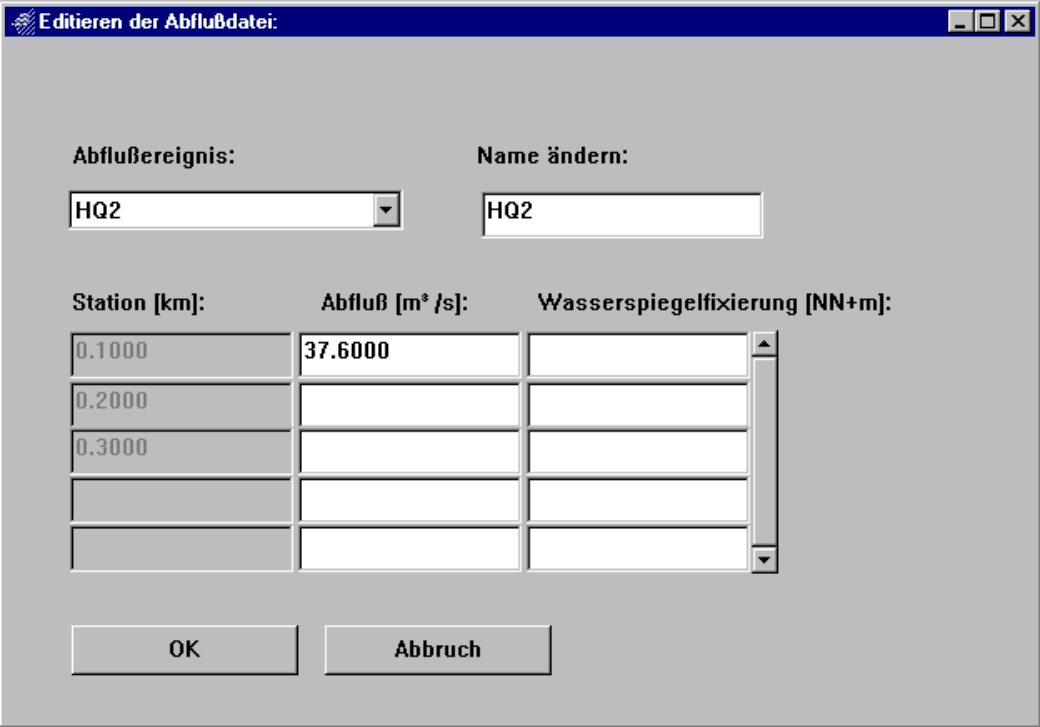
\includegraphics[width=0.7\textwidth]{AbflussdateiEditieren}
   \caption{Der Dialog zum Editieren der Abflu{\ss}datei}
   \label{Einstieg Abb AbflussdateiEditieren}
\end{figure}

Das Dialogfenster \dialog{Editieren der Abflu{\ss}datei} ist wie folgt aufgebaut: Links oben befindet sich ein Listenfeld
mit allen definierten Abflu{\ss}zust\"{a}nden. Solange Sie noch keine Abflu{\ss}datei erstellt haben, finden sich hier lediglich
die Eintr\"{a}ge \afz{neu}. Neben dem Listenfeld ist ein Editierfeld eingef\"{u}gt, in dem Sie die Bezeichnung f\"{u}r den jeweils
im Listenfeld angezeigten Abflu{\ss}zustand neu definieren k\"{o}nnen. Hier vergeben Sie also f\"{u}r den bislang unbenannten
Abflu{\ss}zustand einen neuen Namen (z.B. HQ5), indem Sie diesen \"{u}berschreiben. Der Name mu{\ss} mindestens zwei Zeichen
umfassen. In der Abflu{\ss}tabelle der unteren Bildh\"{a}lfte k\"{o}nnen Sie schlie{\ss}lich Abflu{\ss}werte f\"{u}r dieses Abflu{\ss}ereignis an
s\"{a}mtlichen Stationen, die in Ihrer Strangtabelle definiert wurden, eingeben. Es m\"{u}ssen mindestens zwei Stationen
definiert sein.

Geben Sie bitte nur an den Stationen Werte ein, an denen sich der Abflu{\ss} gegen\"{u}ber der vorherigen Station \"{a}ndert. Die
Abflu{\ss}-Felder von Stationen, an denen sich der Abflu{\ss} nicht \"{a}ndert, k\"{o}nnen leer bleiben. Allerdings mu{\ss} insgesamt an
mindestens einer (der kleinsten) Station ein Abflu{\ss} eingegeben werden.

Falls Sie mehrere Abflu{\ss}ereignisse f\"{u}r einen Zustand definieren m\"{o}chten, w\"{a}hlen Sie aus dem Listenfeld
\feld{Abflu{\ss}ereignis} \afz{neu}. Anschlie{\ss}end erhalten Sie wieder eine neue, zun\"{a}chst noch leere Tabelle, in die Sie
wiederum Abflu{\ss}werte eingeben k\"{o}nnen. Dieser Vorgang ist so oft zu wiederholen, wie Abflu{\ss}zust\"{a}nde definiert werden
sollen. S\"{a}mtliche definierten Abflu{\ss}ereignisse werden schlie{\ss}lich im Listenfeld angezeigt. Die angezeigte Tabelle bezieht
sich auf das jeweils im Listenfeld angezeigte Abflu{\ss}ereignis. Bei der Eingabe der Steuerdaten f\"{u}r die
Spiegellinienberechnung k\"{o}nnen Sie sp\"{a}ter eines dieser Ereignisse ausw\"{a}hlen.

Neben den Abfl\"{u}ssen k\"{o}nnen an den einzelnen Stationen auch Wasserspiegelfixierungen (gemessene Wasserspiegelh\"{o}hen)
eingegeben werden. Die eingegebenen Werte werden im Rahmen der Spiegellinienberechnung sp\"{a}ter sowohl in die L\"{a}ngs- wie
auch in die Querprofildatei eingetragen und k\"{o}nnen so mit den berechneten Werten verglichen werden.

\subsubsection{Beispiel}
Legen sie nun f\"{u}r die in der folgenden Tabelle angegebenen Abflu{\ss}ereignisse eine Abflu{\ss}datei an. Schlie{\ss}en Sie dazu
zun\"{a}chst alle noch ge\"{o}ffneten Dialogfenster.
\begin{quote}
   \begin{tabular}{p{4cm}p{1.5cm}p{1.5cm}p{1.5cm}p{1.5cm}p{1.5cm}}
      Abflu{\ss}ereignis:                & HQ1    & HQ2    &  HQ3   &  HQ4   &  HQ5   \\
      Abflu{\ss} in $\mathrm{[m^3/s]}$:  & $36,6$ & $37,6$ & $38,6$ & $39,6$ & $40,6$
   \end{tabular}
\end{quote}
W\"{a}hlen Sie aus dem Men\"{u} \menu{\marrow Zustand} das Untermen\"{u} \menu{\marrow Abflu{\ss}daten/Wasserspiegelfixie\-rungen}. In den
aufgerufenen Dialog geben Sie im Feld \feld{Name \"{a}ndern} die Bezeichnung f\"{u}r das Abflu{\ss}ereignis \afz{HQ1} ein. Der Wert
f\"{u}r den Abflu{\ss} an der Station $0,10\unit{km}$ betr\"{a}gt $36,6\unit{m^3/s}$.
\begin{quote}
   \begin{tabular}{ll}
      Name \"{a}ndern:                       &  \beisp{HQ1} \\
      Abflu{\ss} an Station $0,10\unit{km}$: &  36,6
   \end{tabular}
\end{quote}
\"{O}ffnen Sie, nachdem Sie den Wert eingetragen haben, das Listenfeld und w\"{a}hlen Sie \afz{neu}. Sie erhalten eine neue
Abflu{\ss}tabelle in der Sie mit der Eingabe fortfahren.

\subsection{Die Verlustdatei}
Zu den Randbedingungen einer Wasserspiegellagenberechnung geh\"{o}ren auch lokale Verluste. Diese k\"{o}nnen unter anderem durch
pl\"{o}tzliche Querschnitts\"{a}nderungen hervorgerufen werden. Diese Verluste werden in einer eigenen Verlustdatei gespeichert.
N\"{a}here Erl\"{a}uterungen zum Umgang mit Einzelverlusten enthalten die Abschnitte~\ref{Fortgeschrittene Subsec Einzelverluste}
und~\ref{Fortgeschrittene Subsec Einstellungen}.


\clearpage
%%%%%%%%%%%%%%%%%%%%%%%%%%%%%%%%%%%%%%%%%%%%%%%%%%%%%%%%%%%%%%%%%%%%%%%%%%%%%%%%%%%%%%%%%%%%%%%%%%%%%%%%%%%%%%%%%%%%%%%%%%%%
\section{Berechnen}
%%%%%%%%%%%%%%%%%%%%%%%%%%%%%%%%%%%%%%%%%%%%%%%%%%%%%%%%%%%%%%%%%%%%%%%%%%%%%%%%%%%%%%%%%%%%%%%%%%%%%%%%%%%%%%%%%%%%%%%%%%%%

\subsection{Fliessgesetze}
\label{Einstieg Subsec Fliessgesetze}

Das grundlegende Verfahren zur Berechnung des Wasserspiegels mit dem \autor{Bernoulli}'schen Energieh\"{o}henvergleich ist in
Abschnitt~\ref{Einfuehrung Subsec TheoretischeGrundlagen} beschrieben. Zur Ermittlung des Energieliniengef\"{a}lles bietet
\wspwin{} dem Anwender sieben Berechnungsmethoden, die alle auf den Flie{\ss}gesetzen von \autor{Manning-Strickler} bzw.
\autor{Prandtl-Colebrook} beruhen.

\subsubsection{Die Theorie nach Manning-Strickler}
Wird die Berechnung der Reibungsverluste nach \autor{Manning-Strickler} durchgef\"{u}hrt, so werden die folgenden
Berechnungsans\"{a}tze nach \cite{FelkelCanisius} verwendet. Ber\"{u}cksichtigt wird jeweils nur eine Rauheit f\"{u}r linkes Vorland,
Flu{\ss}bett und rechtes Vorland. Sind mehr als drei Rauheiten im Profil angegeben, so erfolgen Mittelungen f�r die Werte in den jeweiligen Teilabflu{\ss}querschnitten.
\begin{equation}
   v = k_{ST} \cdot r_{hy}^{2/3} \cdot I_E^{1/2}
\end{equation}
Hydraulische Radien $r_{hy,j}$:
\begin{equation}
   \label{Einstieg Gl HydraulRadius}
   r_{hy,L} = A_L / U_L  \qquad  r_{hy,F} = A_F / U_F  \qquad  r_{hy,R} = A_R / U_R
\end{equation}
Die spezifischen Geschwindigkeiten $w_j$ in $\mathrm{[m/s]}$ betragen:
\begin{equation}
   \label{Einstieg Gl SpezifGeschwindigkeit}
   \begin{split}
      w_L &= k_{ST} \cdot r_{hy}^{2/3} \cdot (l_F/l_L)^{1/2} \\
      w_F &= k_{ST} \cdot r_{hy}^{2/3} \\
      w_R &= k_{ST} \cdot r_{hy}^{2/3} \cdot (l_F/l_R)^{1/2}
   \end{split}
\end{equation}
Hydraulische Leitwerte $C_j$ in $\mathrm{[m^3/s]}$:
\begin{equation}
   C_L = A_L \cdot w_L  \qquad  C_F = A_F \cdot w_F  \qquad  C_R = A_R \cdot w_R
\end{equation}
Gesamtabflu{\ss} $Q$ in $\mathrm{[m^3/s]}$:
\begin{equation}
   Q = \sum C_j \cdot I_E^{1/2}
      \label{Einstieg Gl Gesamtabfluss}
\end{equation}
Teilgeschwindigkeiten $v_j$ in $\mathrm{[m/s]}$:
\begin{equation}
   v_L = w_L \cdot I_E^{1/2}  \qquad  v_F = w_F \cdot I_E^{1/2}  \qquad  v_R = w_R \cdot I_E^{1/2}
\end{equation}
Teilabfl\"{u}sse $Q_j$ in $\mathrm{[m^3/s]}$:
\begin{equation}
   Q_L = v_L \cdot A_L  \qquad  Q_F = v_F \cdot A_F  \qquad  Q_R = v_R \cdot A_R
\end{equation}
Geschwindigkeitsverteilungsbeiwert  $\alpha$ (\autor{Coriolis}-Beiwert):
\begin{equation}
   \label{Einstieg Gl Geschwindigkeitsverteilung}
   \alpha = \frac{1}{A_{ges}} \cdot \sum \left( \frac{v_j^3 \cdot A_j}{v_m^3} \right)
\end{equation}
Impulsstromverteilungsbeiwert $\alpha'$ (\autor{Boussinesq}-Beiwert):
\begin{equation}
   \label{Einstieg Gl Impulsstromverteilung}
   \alpha' = \frac{1}{A_{ges}} \cdot \sum \left( \frac{v_j^2 \cdot A_j}{v_m^2} \right)
\end{equation}
Geschwindigkeitsh\"{o}he $h_k$ in $\mathrm{[m]}$:
\begin{equation}   h_k = \alpha \cdot \frac{v_m^2}{2g}
\end{equation}
\autor{Froud}'sche Zahl $Fr$:
\begin{equation}
   \label{Einstieg Gl Froudezahl}
   Fr = \frac{\sqrt{\alpha} \cdot v_{ges}}{\sqrt{g \cdot A_{ges}/b_{ges}}}
\end{equation}


\subsubsection{Die Theorie nach Prandtl-Colebrook}
Im Falle der Anwendung des allgemeinen Flie{\ss}gesetzes nach
\autor{Prandtl-Colebrook} \cite{DVWK1991} gilt f\"{u}r den vollkommen rauhen Bereich:
\begin{equation}
   v = \sqrt{\frac{8g \cdot r_{hy} \cdot I_E}{\lambda}}
\end{equation}
mit
\begin{equation}
   \frac{1}{\lambda} = 2\lg \left( \frac{14,84 \cdot r_{hy}}{k_S} \right)
      \label{Einstieg Gl LambdaBeiwert}
\end{equation}
ach entsprechender Umformung der Gleichung f\"{u}r den Reibungswert ergeben sich folgende Berechnungsans\"{a}tze f\"{u}r die
Hilfsgr\"{o}{\ss}en wobei die Rauheiten $k_{S,j}$  in $\mathrm{m}$ einzusetzen sind:
\begin{equation}
  \begin{split}
      w_L &= 2\sqrt{8g} \cdot \lg(14,84 \cdot r_{hy,L}/k_{S,L}) \cdot (r_{hy,L} \cdot l_F/l_L)^{1/2} \\
      w_F &= 2\sqrt{8g} \cdot \lg(14,84 \cdot r_{hy,F}/k_{S,F}) \cdot r_{hy,L}^{1/2} \\
      w_R &= 2\sqrt{8g} \cdot \lg(14,84 \cdot r_{hy,R}/k_{S,R}) \cdot (r_{hy,R} \cdot l_F/l_R)^{1/2}
   \end{split}
\end{equation}
Wie schon bei dem Flie{\ss}gesetz nach \autor{Manning-Strickler} rechnet auch der Ansatz nach \autor{Prandtl-Colebrook} mit
nur drei Rauheiten. Alle \"{u}brigen Berechnungsans\"{a}tze zur Bestimmung der hydraulischen Kennwerte eines Profils sind
dieselben wie vorher. F\"{u}r den Abflu{\ss} im geschlossenen Profil (Durchla{\ss}) wird das vollst\"{a}ndige Widerstandsgesetz von
\autor{Prandtl-Colebrook} \cite{PressSchroeder}, das auch im \"{U}bergangsbereich gilt, angewendet. Die L\"{o}sung des
impliziten Widerstandsgesetzes erfolgt durch \autor{Newton}-Iteration.

\subsubsection{Theorie nach Einstein (Manning-Strickler)}
Die Berechnung basiert auf dem Flie{\ss}gesetz von \autor{Manning-Strickler}. Nach \autor{Einstein} kann bei Anwendung dieses
Flie{\ss}gesetzes eine durchschnittliche Rauheit im Profil ohne Iteration berechnet werden.
\begin{equation}
   k_{ST,ges} = \left( \frac{U_{ges}}{\sum \left(U_i/k_{ST,i}^{3/2} \right)}\right)^{2/3}
\end{equation}
Dieser Ansatz f\"{u}r geometrisch einheitliche Profile wird hier sinngem\"{a}{\ss} auf die Teilabflu{\ss}querschnitte des gegliederten
Querschnitts \"{u}bertragen, d.h. die Durchschnittsrauheiten werden getrennt f\"{u}r Vorl\"{a}nder und Flu{\ss}bett berechnet.

\subsubsection{Theorie nach Prandtl-Colebrook + Bewuchs nach Kaiser}
Basierend auf dem Flie{\ss}gesetz von \autor{Prandtl-Colebrook} hat \autor{Kaiser} eine Theorie entwickelt, die mit Hilfe der
spezifischen Vegetationsanstr\"{o}mfl\"{a}che $\omega_P \mathrm{[m]}$  Bewuchs be\-r\"{u}ck\-sich\-tigt (siehe
Abschnitt~\ref{Sonderprofile Subsec Kaiser}). Unabh\"{a}ngig davon k\"{o}nnen mehrere Einzelrauheiten $k_S \mathrm{[m]}$ pro
Teilabflu{\ss}querschnitt angegeben werden.

Die Berechnung der Durchschnittsrauheiten bzw. mittleren Rauheitsbeiwerten gestaltet sich bei der Anwendung der
Flie{\ss}gesetze nach \autor{Prandtl-Colebrook} etwas aufwendiger. Da die Widerstandsbeiwerte $\lambda_i$ von den
hydraulischen Radien abh\"{a}ngen, die zugeordneten Teilfl\"{a}chen jedoch nicht bekannt sind, ist nur eine iterative Berechnung
des Gesamtwiderstandsbeiwertes m\"{o}glich. Der mittlere Rauheitsbeiwert kann nach~\cite{SchroederW} wie folgt ermittelt
werden:
\begin{equation}
   \lambda_{ges} = \frac{ \sum \left(U_i \cdot \lambda_i \right)}{U_{ges}}
      \label{Einstieg Gl LambdaKaiser}
\end{equation}
In einem ersten Schritt werden die Widerstandsbeiwerte $\lambda_i$ mit dem hydraulischen Radius des gesamten
Profilabschnittes bestimmt. So lassen sich nach Gleichung~\ref{Einstieg Gl LambdaKaiser} die hydraulischen Teilradien
berechnen. Werden diese in Gleichung~\ref{Einstieg Gl LambdaBeiwert} eingesetzt, ergeben sich die einzelnen
Widerstandsbeiwerte $\lambda_i$. Die Berechnung wird dann abgebrochen, wenn sich der Gesamtwiderstandsbeiwert nach
Gleichung~\ref{Einstieg Gl LambdaKaiser} nicht mehr \"{a}ndert.


\subsubsection{Theorie nach Prandtl-Colebrook + Bewuchs nach Nuding}
Die Theorie nach \autor{Nuding} ber\"{u}cksichtigt ebenfalls den Bewuchs. Hierf\"{u}r m\"{u}ssen die Bewuchsdurchmesser $D_P$ sowie
die Bewuchsabst\"{a}nde $a_x$ in und $a_y$ quer zur Flie{\ss}richtung angegeben werden (siehe Abschnitt~\ref{Sonderprofile Subsec
Nuding}). Unterschiedliche Einzelrauheiten werden ber\"{u}cksichtigt.

\subsubsection{Theorie nach Prandtl-Colebrook + Bewuchs nach Mertens}
Neben unterschiedlichen Einzelrauheiten werden auch Bewuchsabst\"{a}nde und Bewuchsdurchmesser ber\"{u}cksichtigt (siehe
Abschnitt~\ref{Sonderprofile Subsec Mertens}).

\subsubsection{Theorie nach Prandtl-Colebrook + Bewuchs nach Pasche}
Wie schon bei der Theorie nach \autor{Mertens} werden unterschiedlichen Einzelrauheiten, Bewuchsabst\"{a}nde und
Bewuchsdurchmesser ber\"{u}cksichtigt (siehe Abschnitt~\ref{Sonderprofile Subsec Pasche}).


\subsection{Eingabe der Steuerdaten}

Um die Steuerdaten f\"{u}r die Spiegellinienberechnung anzugeben, w\"{a}hlen Sie aus dem Men\"{u} \menu{\marrow \underline{B}erechnung
\marrow \underline{S}piegellinienberechnung}. Beachten Sie, da{\ss} zuvor eine Zustandsdatei ausgew\"{a}hlt sein mu{\ss}. Sofern sie
nicht schon einmal Daten f\"{u}r die Berechnung angegeben haben, erscheint die Meldung, da{\ss} noch keine Steuerdaten vorhanden
sind.
\begin{figure}[hbt]
   \centering
   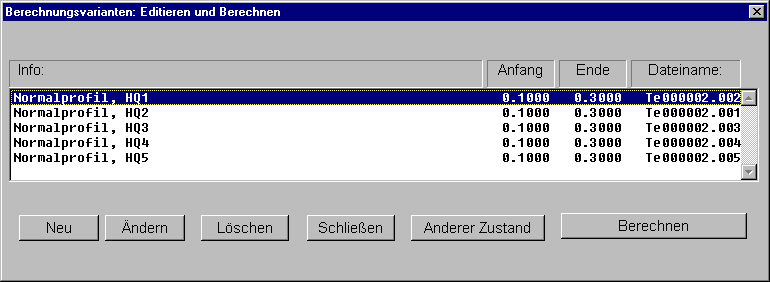
\includegraphics[width=1.0\textwidth]{AuswahlBerechnungsvarianten}
   \caption{Dialogmaske zur Auswahl und zum \"{A}ndern der Berechnungsvarianten}
   \label{Einstieg Subsec AuswahlBerechnungsvarianten}
\end{figure}

Mit Hilfe der Schaltfl\"{a}che \schalter{Neu} gelangen Sie in die Maske \dialog{Steuerdaten}. Hier finden Sie vier
Registerkarten in denen Sie Einstellungen zur Art und Weise der Berechnung, zu Randbedingungen und zur Ausgabeform treffen
k\"{o}nnen. \"{U}ber die Schaltfl\"{a}che \schalter{andere Wahl} k\"{o}nnen sie die Zustandsdatei wechseln, f\"{u}r die die Steuerdaten
vereinbart werden sollen.

Wurde bereits im Vorfeld eine Berechnung durchgef\"{u}hrt, gelangen sie in das Dialogfenster \dialog{Berechnungsvarianten:
Editieren und Berechnen} (Abbildung~\ref{Einstieg Subsec AuswahlBerechnungsvarianten}). Hier haben sie die M\"{o}glichkeit
vorhandene Berechnungsvarianten auszuw\"{a}hlen, zu \"{a}ndern oder neue Berechnungsvarianten zu erstellen. Die Zustandsdatei kann
hier \"{u}ber die Schaltfl\"{a}che \schalter{anderer Zustand} gewechselt werden.

F\"{u}r eine Berechnungsvariante m\"{u}ssen zun\"{a}chst die Basisdaten vereinbart werden. Ganz oben auf der entsprechenden
Registerkarte (Abbildung~\ref{Einstieg Subsubsec Basisdaten}) erscheint ein Feld in dem Sie einen Text mit bis zu
60~Zeichen zu Ihrer Berechnungsvariante eingeben k\"{o}nnen. Darunter l\"{a}{\ss}t sich der Berechnungsabschnitt einschr\"{a}nken. Die
Listenfelder enthalten alle von Ihnen bei der Profileingabe angegebenen Stationen. Voreingestellt sind zun\"{a}chst das
Anfangs- und Endprofil Ihrer bei der Profileingabe festgelegten Kilometrierung. Beachten Sie bei der Eingabe bitte, da{\ss}
das Anfangsprofil stets flu{\ss}ab liegt.

Liegt bezogen auf den Anfangswasserspiegel schie{\ss}ender Abflu{\ss} vor, so mu{\ss} dies \"{u}ber die Checkbox \checkbox{schie{\ss}ender
Abflu{\ss}} angegeben werden. Die Berechnung beginnt dann am OW-Profil.

Um eine Wasserspiegellagenberechnung durchf\"{u}hren zu k\"{o}nnen, mu{\ss} der Wasserspiegel im Anfangsprofil entweder zahlenm\"{a}{\ss}ig
bekannt sein, oder sich aus einer vorgegebenen hydraulischen Randbedingung berechnen lassen. Das Anfangsprofil ist je nach
Flie{\ss}zustand das unterste Profil f\"{u}r den str\"{o}menden bzw. das oberste f\"{u}r den schie{\ss}enden Abflu{\ss}. F\"{u}r die Anfangsbedingung
kann demnach gew\"{a}hlt werden:
\begin{description}
   \item [Bekannte Wasserstand-Abflu{\ss}-Beziehung:]
      Die Wasserspiegellage kann direkt in das Feld \feld{Anfangswasserspiegel} eingegeben werden. Dies trifft kann
      beispielsweise auf bewegliche Wehre mit einem fest vorgegebenen Stauziel zu. In diesem Fall legen Sie das
      Anfangsprofil direkt oberhalb des Wehres. Der Anfangswasserstand entspricht dann dem Stauziel.
   \item [Querschnitt oberhalb eines Flie{\ss}wechsels:]
      An einem Flie{\ss}wechsel tritt zwangsl\"{a}ufig die Grenztiefe (\"{U}bergang Str\"{o}men - Schie{\ss}en) auf. Diese kann mit Hilfe des
      Extremalprinzips im Anfangsprofil des Berechnungsabschnitts iterativ berechnet werden. Markieren Sie dazu
      \checkbox{Grenztiefe}.
   \item[Querschnitt mit ann\"{a}hernd gleichf\"{o}rmigem Abflu{\ss}:]
      Aktivieren Sie den Punkt \checkbox{sta\-tio\-n\"{a}r gleichf\"{o}rmig}, wird die Normalwassertiefe iterativ aus dem
      angegebenen Energieliniengef\"{a}l\-le (absolut) im ersten Profil berechnet.
   \item[Querschnitt oberhalb eines festen Wehres mit vollkommenem \"{U}berfall:]
      Der An\-fangs\-wasserstand wird hier mit Hilfe der \autor{Poleni}-Formel aus der Kronenh\"{o}he des Wehres und der
      \"{U}berfallh\"{o}he berechnet. Markieren Sie die Checkbox \checkbox{Wehr am Anfang}.
\end{description}

F\"{u}r den Fall, da{\ss} keine der beschriebenen hydraulischen Randbedingungen zutreffen, ist die Berechnungsstrecke flu{\ss}abw\"{a}rts
zu verl\"{a}ngern. Man sch\"{a}tzt einen Anfangswasserstand und f\"{u}hrt eine Wasserspiegellagenberechnung durch. Der bei der
Sch\"{a}tzung gemachte Fehler wirkt sich nach oberstrom von Profil zu Profil (abh\"{a}ngig von Gef\"{a}lle und Flie{\ss}geschwindigkeit)
immer weniger aus, so das bei entsprechender Verl\"{a}ngerung der vorangestellten Berechnungsstrecke der Einflu{\ss} auf den
Anfangswasserstand des eigentlich betrachteten Flu{\ss}abschnitts vernachl\"{a}ssigbar gering ist.
\begin{figure}[bth]
   \centering
   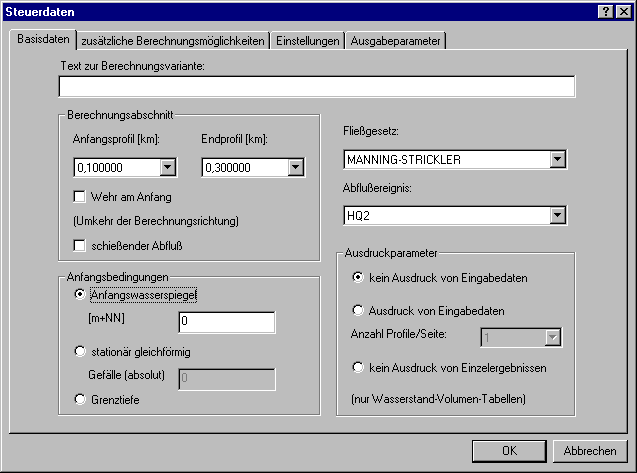
\includegraphics[width=1.0\textwidth]{Basisdaten}
   \caption{Dialog zum Festlegen der Basisdaten f\"{u}r die Spiegellinienberechnung}
   \label{Einstieg Subsubsec Basisdaten}
\end{figure}

Voraussetzung f\"{u}r diese Vorgehensweise ist jedoch, da{\ss} der neue Ausgangswasserstand nicht im Staubereich einer noch weiter
unterhalb gelegenen St\"{o}rung liegt. Zur Probe f\"{u}r die richtige \"{U}berl\"{a}nge wird die Berechnung mit einem anderen
Anfangswasserstand wiederholt, wobei sich angen\"{a}hert derselbe Wert f\"{u}r den Wasserspiegel des eigentlichen Anfangsprofils
ergeben mu{\ss}.

Auf der rechten Seite der Registerkarte \dialog{Basisdaten} finden sie ein Listenfeld zur Auswahl der in
Abschnitt~\ref{Einstieg Subsec Fliessgesetze} n\"{a}her beschriebenen Flie{\ss}gesetze. Darunter k\"{o}nnen sie ein Abflu{\ss}ereignis
aus Ihrer Abflu{\ss}datei (Abschnitt~\ref{Einstieg Subsec Abflussdatei}) ausw\"{a}hlen, f\"{u}r das die Berechnung durchgef\"{u}hrt
werden soll. Beachten Sie bei der Auswahl des Flie{\ss}gesetzes, da{\ss} im Vorfeld die f\"{u}r die Berechnung zugeh\"{o}rigen
Rauheiten nach Abschnitt~\ref{Einstieg Subsec Rauheit} definiert sind. Es kann z.B. keine Berechnung nach der
Flie{\ss}theorie von \autor{Manning-Strickler} auf Grundlage der \autor{Darcy-Weisbach}'schen Rauheiten erfolgen.

Bez\"{u}glich der Darstellung der Ergebnistabelle k\"{o}nnen hier weiterhin folgende Einstellungen getroffen werden:
\begin{description}
   \item [Kein Ausdruck von Eingabedaten:]
      Es werden nur die Berechnungsergebnisse ausgegeben.
   \item [Ausdruck von Eingabedaten:]
      Dem Ergebnisausdruck werden die Eingabedaten vorangestellt. Die Anzahl der Profile pro Seite kann zus\"{a}tzlich
      festgelegt werden.
   \item [Kein Ausdruck von Einzelergebnissen:]
      Sofern Sie neben der normalen Berechnung die Ausgabe der Abflu{\ss}-Wasserstand-Volumen-Tabellen gew\"{a}hlt haben, haben
      Sie hier die M\"{o}glichkeit nur die Ergebnisse der Tabellen ohne die normale Wasserspiegellagenberechnung auszugeben.
\end{description}

Die Funktionen auf den Registerkarten \dialog{zus\"{a}tzliche Berechnungsm\"{o}glichkeiten}, \dialog{Einstellungen} und
\dialog{Ausgabeparameter} werden im Kapitel~\ref{Fortgeschrittene} erl\"{a}utert.


\subsubsection{Beispiel Steuerdaten}

Legen Sie im folgenden f\"{u}r den \afz{Testbach} eine Berechnungsvariante an. Schlie{\ss}en Sie dazu zun\"{a}chst alle noch
ge\"{o}ffneten Dialogfenster. W\"{a}hlen Sie aus dem Men\"{u} \menu{\marrow \underline{B}erechnen \marrow
\underline{S}piegellinienberechnung}.

Da im Vorfeld noch keine Steuerdaten vereinbart wurden, f\"{u}hrt man sie zun\"{a}chst in den Dialog zur Erstellung einer neuen
Berechnungsvariante. In die Registerkarte \dialog{Basisdaten} tragen Sie bitte ein:
\begin{quote}
   \begin{tabular}{ll}
      Text zur Berechnungsvariante:       &  \beisp{Normalprofil, HQ1} \\
      Anfangsprofil:                      &  \beisp{0,1} \\
      Endprofil:                          &  \beisp{0,3} \\
      Flie{\ss}gesetz:                        &  \beisp{Prandtl-Colebrook} \\
      Abflu{\ss}ereignis:                     &  \beisp{HQ1} \\
      Anfangswasserspiegel:               &  \beisp{158,0} \\
   \end{tabular}
\end{quote}
F\"{u}r die Ausdrucksparameter geben Sie \afz{kein Ausdruck von Eingabedaten} an. Speichern Sie die Eingaben mit
\schalter{OK}.


\subsection{Die Berechnung starten}

Nachdem Sie die Dialogmaske zum Editieren der Steuerdaten mit \schalter{OK} verlassen und damit alle Eingabedaten
gespeichert haben, gelangen Sie automatisch in ein Fenster, in dem s\"{a}mtliche bereits angelegten Berechnungsvarianten
mit ihrer Kennzeichnung, dem Anfangs- und Endprofil des Berechnungsabschnitts und dem Dateinamen aufgelistet sind
(Abbildung~\ref{Einstieg Subsec AuswahlBerechnungsvarianten}). Diese \"{U}bersicht wird an sp\"{a}teren Stellen (z.B. Auswahl
des L\"{a}ngsschnitts zum Plotten) noch mehrfach erscheinen. Aus dieser \"{U}bersichtsmaske heraus k\"{o}nnen sie bereits angelegte
Berechnungsvarianten jederzeit wieder \"{a}ndern, bearbeiten, l\"{o}schen oder neue Varianten anlegen.

Diese Berechnungsvariantenverkn\"{u}pfungsdatei ist stets einer Zustandsdatei zugeordnet. \"{U}ber die Schaltfl\"{a}che
\schalter{Anderer Zustand} k\"{o}nnen Sie auch Varianten aus anderen Zust\"{a}nden bearbeiten. \"{U}ber \schalter{Schlie{\ss}en}
verlassen Sie die Maske.

Den eigentlichen Berechnungsvorgang starten Sie \"{u}ber den Schalter \schalter{Berechnen}. Sie k\"{o}nnen eine oder mehrere
Varianten zur Berechnung markieren (STRG + Mausklick bzw. STRG + Pfeiltaste) und ausw\"{a}hlen.

Beim Berechnungsvorgang wird ein externes Programm gestartet. Nach Abschlu{\ss} der Berechnung erhalten Sie eine R\"{u}ckmeldung.
Der Benutzer kann nach erfolgreicher Berechnung die Ergebnisdateien im Unterverzeichnis
\datei{\textbackslash dath} einsehen.

Im Rahmen der Berechnung werden in den L\"{a}ngs- und Querprofilen automatisch alte berechnete Wasserspiegellagen gel\"{o}scht und
die aktuellen Werte eingetragen. Bei Markierung und Berechnung mehrerer Varianten werden auch mehrere Wasserspiegel
grafisch dargestellt.


\subsubsection{Beispiel Berechnung starten}

Legen Sie zun\"{a}chst vier weitere Berechnungsvarianten f\"{u}r die Abflu{\ss}ereignisse HQ2, HQ3, HQ4 und HQ5 an. Markieren Sie
diese im Anschlu{\ss}, indem sie die STRG-Taste gedr\"{u}ckt halten und die Varianten anklicken. Starten Sie die Berechnung
\"{u}ber den Schalter \schalter{Berechnen}.


\clearpage
%%%%%%%%%%%%%%%%%%%%%%%%%%%%%%%%%%%%%%%%%%%%%%%%%%%%%%%%%%%%%%%%%%%%%%%%%%%%%%%%%%%%%%%%%%%%%%%%%%%%%%%%%%%%%%%%%%%%%%%%%%%%
\section{Berechnungsergebnisse einsehen}
%%%%%%%%%%%%%%%%%%%%%%%%%%%%%%%%%%%%%%%%%%%%%%%%%%%%%%%%%%%%%%%%%%%%%%%%%%%%%%%%%%%%%%%%%%%%%%%%%%%%%%%%%%%%%%%%%%%%%%%%%%%%

\subsection{Der WspWin-Editor}

Der Untermen\"{u}punkt \menu{\marrow Tabelle} des Men\"{u}s \menu{\marrow Ergebnisse} erm\"{o}glicht es Ihnen, jederzeit die
tabellarischen Ergebnisse der Spiegellinienberechnung (aber auch Auswertungsergebnisse, Fehlermeldungen und beliebige
Textdateien im ASCII-Format (s.u.)) einzusehen, zu formatieren und zu drucken.

Nachdem Sie den Men\"{u}punkt gew\"{a}hlt haben, erscheint zun\"{a}chst die Maske zur Auswahl der Berechnungsvariante. Es wird ein
neues Programm, n\"{a}mlich der \wspwin{}-Editor gestartet und Ihr Berechnungsergebnis angezeigt. Der Editor ist den \"{u}blichen
Win\-dows-Konventionen entsprechend aufgebaut (vgl. z.B. Wordpad.exe).
\begin{hinweis}
   Wenn Sie im Men\"{u} \menu{\marrow E\underline{x}tras \marrow \underline{O}ptionen} in der Registerkarte
   \dialog{Verzeichnisse} den Pfad der \datei{Editor.exe} angeben, k\"{o}nnen Sie den \wspwin{}Editor auch direkt \"{u}ber das
   Men\"{u} \menu{\marrow \underline{E}rgebnisse \marrow \underline{E}ditor} starten. Sie finden die Datei im
   \wspwin{}-Installationsverzeichnis. In gleicher Weise kann aber auch ein weiterer Editor integriert werden.
\end{hinweis}

M\"{o}chten Sie eine andere Ergebnis- oder Protokolldatei im Editor einsehen (\menu{\marrow \underline{D}atei \marrow
\underline{\"{O}}ffnen...}), erscheint die in Abbildung~\ref{Einstieg Abb EditorDateiOeffnen} dargestellte Maske, die zun\"{a}chst
s\"{a}mtliche Gew\"{a}sser des aktuellen Projektes auflistet. Durch Klicken auf das +-K\"{a}stchen werden s\"{a}mtliche Zust\"{a}nde
dargestellt, die ihrerseits wieder aufgeklappt werden k\"{o}nnen, um zu entscheiden, ob Berechnungsergebnisse oder Ergebnisse
der Auswerteprogramme dargestellt werden sollen. Hat man sich f\"{u}r eine der beiden Varianten entschieden, werden rechter
Hand s\"{a}mtliche vorhandenen Berechnungsvarianten aufgelistet und man kann durch Markierung und Best\"{a}tigung mit
\schalter{OK} eine Variante einsehen. Zus\"{a}tzlich zu den Berechnungsergebnissen werden auch die Fehlerdateien aufgelistet.
Sie k\"{o}nnen ebenfalls mit Hilfe des Editors eingesehen werden.
\begin{figure}[htp]
   \centering
   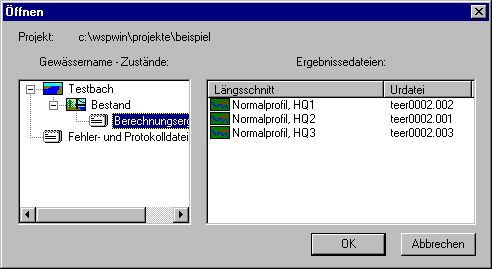
\includegraphics[width=0.8\textwidth]{EditorDateiOeffnen}
   \caption{Datei im Editor \"{o}ffnen}
   \label{Einstieg Abb EditorDateiOeffnen}
\end{figure}

Will man davon abweichend eine beliebige Textdatei \"{u}ber den Standard-Windows-Dialog zur Dateiauswahl \"{o}ffnen, hat man unter
dem Men\"{u}punkt \menu{\marrow \datei{D}atei} zun\"{a}chst das Untermen\"{u} \menu{\marrow Projekt s\underline{c}hlie{\ss}en} zu w\"{a}hlen.
Danach kann man \"{u}ber \menu{\marrow Datei \underline{\"{o}}ffnen} eine beliebige Textdatei \"{o}ffnen und editieren. Ebenso ist es
m\"{o}glich ein anderes Projekt mit Hilfe der Men\"{u}option \menu{\marrow \"{O}ffnen \underline{P}rojekt} auszuw\"{a}hlen.

Der Texteditor stellt bei Ergebnisdateien im ANSI-Format Seitenumbr\"{u}che durch K\"{a}stchen dar. \"{U}ber den Men\"{u}punkt
\menu{\marrow For\-ma\underline{t} \marrow Seitenwechsel} kann an der Stelle, an der sich der Cursor momentan befindet,
ein weiterer Seitenwechsel eingef\"{u}gt werden. Zum L\"{o}schen des Seitenumbruchs entfernen Sie das K\"{a}stchen wieder.
\begin{figure}
   \centering
   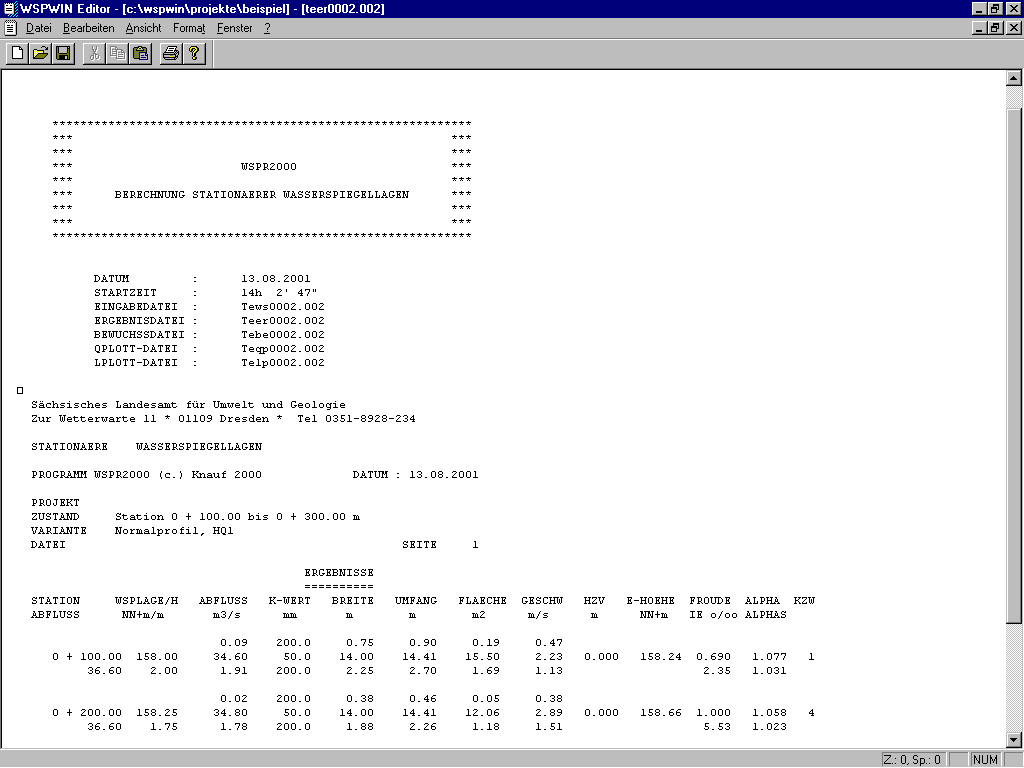
\includegraphics[width=1.0\textwidth]{Editor}
   \caption{Einsehen einer Datei im Texteditor}
   \label{Einstieg Abb Editor}
\end{figure}

Das Men\"{u} \menu{\marrow Forma\underline{t}} bietet weiterhin die M\"{o}glichkeit die Einstellungen f\"{u}r die Schriftart und das
Absatzlayout zu ver\"{a}ndern. Mit Hilfe der Funktion \menu{\marrow OEM$\leftrightarrow$ANSI} kann das Aussehen der Umlaute
und Sonderzeichen, falls erforderlich, ver\"{a}ndert werden.

Die Ergebnisse Ihrer Berechnung k\"{o}nnen auch aus dem Editor heraus gedruckt werden. Nachdem Sie die Men\"{u}folge \menu{\marrow
\underline{D}atei \marrow \underline{D}rucken...} gew\"{a}hlt haben, erscheint der Ihnen aus anderen Windows-Anwendungen
bekannte Dialog in dem Sie Seitenformat, Druckertreiber etc. ausw\"{a}hlen k\"{o}nnen. Standardm\"{a}{\ss}ig werden Ihnen die Optionen der
Systemdruckereinstellung angezeigt. Mit \schalter{OK} starten sie den Druckvorgang, \"{u}ber \schalter{Eigenschaften} nehmen
Sie ggf. weiter Druckereinstellungen vor.


\subsubsection{Beispiel - Einsehen der Berechnungsergebnisse}

Sehen Sie die Berechnungsergebnisse Ihrer ersten Berechnungsvariante ein. W\"{a}hlen Sie dazu aus dem Men\"{u} \menu{\marrow
\underline{E}rgebnisse} den Punkt \menu{\marrow \underline{T}abelle}. Es erscheint die Dialogmaske zur Auswahl einer
Berechnungsvariante. Markieren Sie die Variante \afz{Normalprofil, HQ1} und best\"{a}tigen Sie mit \schalter{OK}.

\begin{hinweis}
   Der \wspwin{}-Editor stellt ein eigenst\"{a}ndiges Programm dar, das auch ohne das Berechnungsprogramm genutzt werden kann.
   Wenn Sie auf Ihrem Desktop eine Verkn\"{u}pfung zu der Datei \datei{Editor.exe} im Installationsverzeichnis vom \wspwin{}
   erstellen, k\"{o}nnen Sie das Programm aus Windows heraus direkt starten. Es ist so m\"{o}glich Dateien und Berechnungsergebnisse
   einzusehen, ohne da{\ss} dazu \wspwin{} aufgerufen werden mu{\ss}.
\end{hinweis}


\subsection{Erl\"{a}uterung der Abk\"{u}rzungen im Ergebnisausdruck}
\label{Einstieg Subsec Ergebnisausdruck}

Der Ergebnisausdruck in der Standardeinstellung zeigt zun\"{a}chst in der ersten Spalte der Tabelle die Stationierung des
Profils. Darunter wird der Gesamtabflu{\ss} in $\unit{[m^3/s]}$ ausgegeben. Die zweite Spalte enth\"{a}lt in der ersten Zeile die
Wasserspiegellage $W$ in $\unit{[NN\!+\!m]}$ bzw. $\unit{[HN\!+\!m]}$. Darunter steht die Wassertiefe in $\unit{[m]}$.

Die darauffolgenden Spalten gliedern sich jeweils in drei Zeilen (vgl. Abbildung~\ref{Einstieg Abb Editor}). In der
ersten Zeile stehen die Werte f\"{u}r das linke Vorland, in der dritten die des rechten Teilabflu{\ss}querschnitts. Die
mittlere Zeile gibt die Werte f\"{u}r den Flu{\ss}schlauch an.
\begin{quote}
   \begin{tabular}{p{0.15\linewidth}p{0.8\linewidth}}
      ABFLUSS \newline  m3\slash s
            &  Teilabflu{\ss} $Q_L$, $Q_F$, $Q_R$ in $\unit{[m^3/s]}$ im Flu{\ss}bett und Vorland, \\[18pt]
      K-WERT \newline m\^{}.33/s
            &  Rauheit $k_{ST,j}~\unit{[m^{1/3}/s]}$ nach \autor{Manning-Strickler} im Teilabflu{\ss}querschnitt oder \\[6pt]
      K-WERT \newline m
            &  Rauheit $k_{S,j} \unit{[m]}$ nach \autor{Darcy-Weisbach} im Teilabflu{\ss}querschnitt \\[6pt]
      BREITE \newline m
            &  Breite des Wasserspiegels in den Vorl\"{a}ndern und im Flu{\ss}schlauch \\[6pt]
      UMFANG \newline m
            &  Benetzer Umfang $U_L$, $U_F$, $U_R$ des jeweiligen Teilabflu{\ss}querschnitts in $\unit{[m]}$, \\[6pt]
      FL\"{A}CHE \newline m2
            &  Flie{\ss}querschnitte $A_L$, $A_F$, $A_R$ der jeweiligen Teilabflu{\ss}querschnitte in $\unit{[m^2]}$, \\[6pt]
      GESCHW \newline m\slash s
            &  Mittlere Flie{\ss}geschwindigkeiten $v_L$, $v_F$, $v_R$ im jeweiligen Teilabflu{\ss}querschnitt in $\unit{[m/s]}$
   \end{tabular}
\end{quote}
Im Anschlu{\ss} an die getrennte Darstellung der Flie{\ss}parameter f\"{u}r Vorl\"{a}nder und Hauptgerinne werden noch verschiedene
Kenngr\"{o}{\ss}en die den gesamten Flie{\ss}querschnitt betreffen ausgegeben.
\begin{quote}
   \begin{tabular}{p{0.15\linewidth}p{0.8\linewidth}}
      HZV \newline m
            &  Errechnete Verlusth\"{o}he $H_{ZV}~\unit{[m]}$ aus den Einzelverlusten an der Station. \\[6pt]
      E-HOEHE \newline NN + m
            &  Die berechnete H\"{o}he $H_E$ der Energielinie in $\unit{[NN\!+\!m]}$ bzw. $\unit{[HN\!+\!m]}$ f\"{u}r den
               Profilquerschnitt wird wiedergegeben \\[6pt]
      FROUDE \newline IE o\slash oo
            &  Die erste Zeile gibt die \autor{Froude}-Zahl zur Kennzeichnung des Flie{\ss}zustandes wieder (s.u.).
               Darunter wird das querschnittsspezifische Energieliniengef\"{a}lle unter Einschlu{\ss} der
               Geschwindigkeitsverteilung (Gleichung~\ref{Einstieg Gl Gesamtabfluss}) ausgegeben. \\[6pt]
      ALPHA \newline ALPHAS
            &  Geschwindigkeitsverteilungsbeiwert $\alpha$ und Impulsstromverteilungsbeiwert $\alpha'$.
   \end{tabular}
\end{quote}

Zur schnellen Orientierung und zur Kontrolle der Berechnungsart wird am rechten Rand der Ergebnislisten f\"{u}r jedes
berechnete Querprofil ein Kennungsparameter $KZW$ ausgegeben, der angibt, mit welchem Unterprogramm gerechnet wurde. In
Normalprofilen kann $KZW$ folgende Werte erhalten.
\begin{quote}
   \begin{tabular}{lp{0.8\linewidth}}
      $KZW =  0$  &  Spiegelh\"{o}he aus Spiegellinieniteration \\
      $KZW =  1$  &  Wasserstand vorgegeben \\
      $KZW =  2$  &  $k$-Wert Berechnung Flu{\ss}bett \\
      $KZW =  3$  &  $k$-Wert Berechnung Vorl\"{a}nder \\
      $KZW =  4$  &  Spiegellage ist gleich der Grenztiefe \\
      $KZW =  5$  &  Spiegellage ist gleich der Normalwassertiefe \\
      $KZW =  6$  &  Wasserstand oberhalb eines vollkommenen \"{U}berfalls \\
      $KZW =  7$  &  Spiegellage aus vorhergehendem Berechnungsabschnitt \\
      $KZW =  8$  &  Pfeilerstau nach \autor{Rehbock} \\
      $KZW =  9$  &  Wasserstand ergibt sich aus erforderlicher Mindestenergie\-h\"{o}he im Durchla{\ss}
   \end{tabular}
\end{quote}
Bei Aufstau in geschlossenen Profilen ohne \"{U}berflutung werden die Kennziffern~10 bis 19 f\"{u}r die Berechnung nach der
Flie{\ss}theorie von \autor{Manning-Strickler} und die Kennziffern~20 bis 29 f\"{u}r die Berechnung nach \autor{Prandtl-Colebrook}
vergeben.
\begin{quote}
   \begin{tabular}{lcc}
      Durchla{\ss}typ                            &  \autor{Strickler} &  \autor{Prandtl-Colebrook} \\[6pt]
      Kreisprofil                            &  $KZW = 10$        &  $KZW = 20$ \\
      Durchla{\ss} mit horizontaler Decke        &  $KZW = 11$        &  $KZW = 21$ \\
      Halbkreis oder Kreissegment            &  $KZW = 12$        &  $KZW = 22$ \\
      Maulprofil DIN~4263                    &  $KZW = 13$        &  $KZW = 23$ \\
      Maulprofil ARMCO Fibel~71              &  $KZW = 14$        &  $KZW = 24$ \\
      Wertetabelle f\"{u}r lineare Interpolation &  $KZW = 15$        &  $KZW = 25$ \\
      Eiprofil DIN~4263                      &  $KZW = 16$        &  $KZW = 26$ \\
      Maulprofil ARMCO Fibel~84              &  $KZW = 17$        &  $KZW = 27$ \\
      Ellipsenprofil ARMCO Fibel~84          &  $KZW = 18$        &  $KZW = 28$ \\
      Super-Span ARMCO Fibel~84              &  $KZW = 19$        &  $KZW = 29$
   \end{tabular}
\end{quote}
Tritt dagegen ein Aufstau mit \"{U}berflutung auf, so nimmt der $KZW$-Wert in Abh\"{a}ngigkeit vom Flie{\ss}gesetz Werte zwischen
30 und 49 an.
\begin{quote}
   \begin{tabular}{lcc}
      Durchla{\ss}typ                            &  \autor{Strickler} &  \autor{Prandtl-Colebrook} \\[6pt]
      Kreisprofil                            &  $KZW = 30$        &  $KZW = 40$ \\
      Durchla{\ss} mit horizontaler Decke        &  $KZW = 31$        &  $KZW = 41$ \\
      Halbkreis oder Kreissegment            &  $KZW = 32$        &  $KZW = 42$ \\
      Maulprofil DIN~4263                    &  $KZW = 33$        &  $KZW = 43$ \\
      Maulprofil ARMCO Fibel~71              &  $KZW = 34$        &  $KZW = 44$ \\
      Wertetabelle f\"{u}r lineare Interpolation &  $KZW = 35$        &  $KZW = 45$ \\
      Eiprofil DIN~4263                      &  $KZW = 36$        &  $KZW = 46$ \\
      Maulprofil ARMCO Fibel~84              &  $KZW = 37$        &  $KZW = 47$ \\
      Ellipsenprofil ARMCO Fibel~84          &  $KZW = 38$        &  $KZW = 48$ \\
      Super-Span ARMCO Fibel~84              &  $KZW = 39$        &  $KZW = 49$
   \end{tabular}
\end{quote}
Die folgenden Kennziffern geben Auskunft \"{u}ber weitere spezielle Berechnungsvarianten
\begin{quote}
   \begin{tabular}{lp{0.8\linewidth}}
   		$KZW =  55$  &  Normalwassertiefe f�r alle Profile \\
      $KZW =  61$  &  \"{U}berfallbeiwert wurde nach \autor{Kandaswany\slash Rouse} berechnet \\
      $KZW =  65$  &  Fl\"{a}chenberechnung nach \autor{Gauss} (Manning-Strickler) \\
      $KZW =  66$  &  Fl\"{a}chenberechnung nach \autor{Gauss} (Prandtl-Colebrook) \\
      $KZW =  70$  &  Streichwehr \\
      $KZW =  71$  &  breitkroniges Wehr \\
      $KZW =  72$  &  dachf\"{o}rmiges Wehr \\
      $KZW =  73$  &  rundkroniges Wehr \\
      $KZW =  74$  &  scharfkantiges Wehr \\
      $KZW =  77$  &  Wehr mit unterschiedlichen Kronenh\"{o}hen
   \end{tabular}
\end{quote}
Bei Teilstrecken von Verzweigungen steht vor der $KZW$-Kennziffer die jeweilige Teilstreckennummer.
\begin{quote}
   $KZW = \mathit{IVZ}*100 + KZW$
\end{quote}
Entspricht die Berechnungsrichtung der Flie{\ss}richtung (schie{\ss}ender Abflu{\ss}), so werden negative Kennziffern vergeben.
\begin{quote}
   \begin{tabular}{lp{0.8\linewidth}}
      $KZW = -1$  &  Wasserstand vorgegeben f\"{u}r schie{\ss}enden Abflu{\ss}, Anfangswasserstand im oberwasserseitigen
                     Anfangsprofil \\
      $KZW = -4$  &  Anfangswasserstand ist gleich der Grenztiefe (schie{\ss}ender Abflu{\ss}) \\
      $KZW = -5$  &  Anfangswasserstand ist gleich der Normalwassertiefe
   \end{tabular}
\end{quote}
Hinter Zahlenwerten k\"{o}nnen zus\"{a}tzliche Kennzeichen auftreten, wie z.B:
\begin{quote}
   \begin{tabular}{ll}
      *  (hinter Fl\"{a}chenwert) &  Inselbildung, Gel\"{a}nde teilweise \"{u}ber WSP \\
      DH (neben WSP-Lage)     &  Druckh\"{o}he, kein freier Wasserspiegel \\
      UE (neben WSP-Lage)     &  Durchla{\ss} wird \"{u}berstr\"{o}mt \\
      ***                     &  Energieh\"{o}he steigt nicht an
   \end{tabular}
\end{quote}
Die \autor{Froude}'sche Zahl gibt den Flie{\ss}zustand im Gerinne wieder. Es bedeuten:
\begin{quote}
   \begin{tabular}{ll}
      $Fr > 1$ &  Schie{\ss}ender Abflu{\ss} \\
      $Fr = 1$ &  Kritischer Abflu{\ss} (Flie{\ss}wechsel) \\
      $Fr < 1$ &  Str\"{o}mender Abflu{\ss} \\
      $Fr = 0$ &  Str\"{o}mung ohne freien Wasserspiegel (Druckabflu{\ss})
   \end{tabular}
\end{quote}

Die Durchstr�mungsart wird durch die Kennziffer KZD gekennzeichnet.

\begin{tabular}{ll}
	\\
	\underline{- mit Einstau der Br�ckenunterkante DKUK, keine �berstr�mung} \\
	Standardberechnung mit Verlustbeiwerte  & 0 \\
	Sch�tzstr�mung nach \autor{Schmidt}			& 1 \\
	Sch�tzstr�mung nach \autor{Knapp}				& 2 \\
	eintauchende Br�ckenplatten nach Naudascher-Medlarz	& 3 \\
	\\
	\underline{- mit �berstr�mung der Br�ckenoberkante DKOK} \\
	Standardberechnung mit Verlustbeiwerte		& 5 \\
	Sch�tzstr�mung nach \autor{Schmidt}	 			&	6 \\
	Sch�tzstr�mung nach \autor{Knapp}					&	7 \\
\end{tabular}

\subsection{Der L\"{a}ngsschnitteditor}
\label{Einstieg Subsec Laengsschnitteditor}

Nachdem Sie eine Spiegellinienberechnung erfolgreich durchgef\"{u}hrt haben, haben Sie unter dem Men\"{u}punkt \menu{\marrow
\underline{E}rgebnisse \marrow \underline{L}\"{a}ngsschnitt einsehen} die M\"{o}glichkeit, das Ergebnis der Berechnung in einer
Grafik einzusehen.
\begin{figure}[hbt]
   \centering
   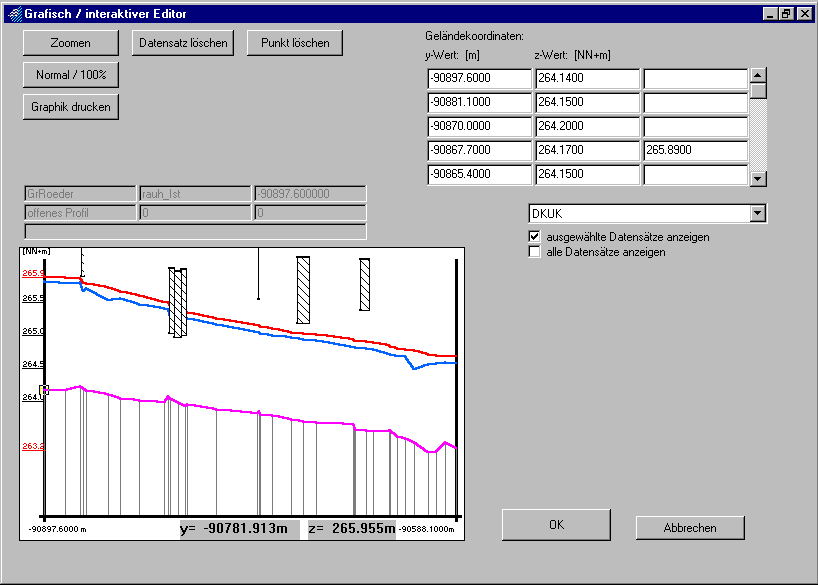
\includegraphics[width=1.0\textwidth]{Laengsschnitteditor}
      \caption{L\"{a}ngsschnitteditor}
      \label{Einstieg Abb Laengsschnitteditor}
\end{figure}

Wenn die Option gew\"{a}hlt wird erscheint, falls noch keine Vernetzungsdatei gew\"{a}hlt wurde, zun\"{a}chst wiederum die
Dialogmaske zur \dialog{Auswahl einer Zustandsdatei}. Anschlie{\ss}end werden Sie zur Auswahl einer Berechnungsvariante
aufgefordert.

W\"{a}hrend der Berechnung wird automatisch eine L\"{a}ngsschnittdatei im BCE-Format erzeugt, die im Grafik-Editor f\"{u}r
L\"{a}ngsschnitte eingesehen und sp\"{a}ter auch geplottet werden kann. Der L\"{a}ngsschnitteditor ist analog zum Grafik-Editor f\"{u}r
Querprofile aufgebaut. Der einzige Unterschied besteht darin, da{\ss} keine neuen Datens\"{a}tze angelegt werden k\"{o}nnen.
Folgende Datens\"{a}tze werden bei L\"{a}ngsschnitten automatisch erzeugt:
\begin{quote}
   \begin{labeling}[~]{Schleppspannung {[N/m2]}}
      \item[Sohlh\"{o}he]                  Lage der Sohle, grafische und alphanumerische Darstellung (magenta Linie)
      \item[B\"{o}schung li.]              Linke B\"{o}schungsoberkante, grafische und alphanumerische Darstellung (gelbe Linie)
      \item[B\"{o}schung re.]              Rechte B\"{o}schungsoberkante, grafische und alphanumerische Darstellung (orange Linie)
      \item[Ausuferung li.]            grafische und alphanumerische Darstellung (hellgr\"{u}ne Linie)
      \item[Ausuferung re.]            grafische und alphanumerische Darstellung (graue Linie)
      \item[Wasserspiegel]             Lage des Wasserspiegels, grafische und alphanumerische Darstellung (blaue Linie)
      \item[Abflu{\ss}]                    Abflu{\ss}, alphanumerisch
      \item[Schleppspannung {[N/m2]}]  Sohlschubspannung, alphanumerisch
      \item[WSP-Breite]                Wasserspiegelbreite, alphanumerisch
      \item[Energieh\"{o}he {[NN+m]}]      Energieh\"{o}he, grafische und alphanumerische Darstellung (rote Linie)
      \item[DKUK]                      Deckenunterkante (nur bei Sonderprofilen), grafische und alphanumerische
                                       Darstellung (schwarz schraffierter Kasten)
      \item[DKOK]                      Deckenoberkante (nur bei Sonderprofilen), grafische und alphanumerische Darstellung
                                       (schwarz schraffierter Kasten)
      \item[Profilart]                 Nummern analog $KZW$ (Abschnitt~\ref{Einstieg Subsec Ergebnisausdruck}, alphanumerisch
      \item[Profilkennung]             Profilkennung, alphanumerisch, 1=LL, 2=FF, 3=RR
      \item[Verzweigung]               Verzweigungskennung, alphanumerisch
      \item[Wasserspiegelfixierung]    grafische und alphanumerische Darstellung (nur wenn in Steuerdaten aktiviert und
                                       unter \menu{\marrow Zustand\marrow Abflu{\ss}daten/Wasserspiegelfixierungen} eingegeben)
      \item[Wasserspiegeldifferenz]    Differenz zwischen gemessenem und berechneten Wasserspiegel.
   \end{labeling}
\end{quote}

Die Datens\"{a}tze \afz{Sohlh\"{o}he}, \afz{B\"{o}schung li.}, \afz{B\"{o}schung re.}, die errechnete Wasserspiegelh\"{o}he sowie bei
entsprechenden Profilen ggf. die H\"{o}he der Deckenoberkante und -unterkante werden grafisch dargestellt. Sofern Sie die
Datens\"{a}tze nicht nur einzeln darstellen m\"{o}chten, haben Sie \"{u}ber das K\"{a}stchen \checkbox{alle Datens\"{a}tze anzeigen} die
M\"{o}glichkeit, sich alle angelegten Datens\"{a}tze parallel anzeigen zu lassen. Sollen nur bestimmte Datens\"{a}tze in der Grafik
angezeigt werden, so ist dies \"{u}ber die Checkbox \checkbox{ausgew\"{a}hlte Datens\"{a}tze anzeigen} m\"{o}glich.  W\"{a}hlen Sie hierzu,
jeden der darzustellenden Parameter explizit nacheinander aus dem Listenfeld mit allen Datens\"{a}tzen an. Diese werden dann
nacheinander in die Grafik \"{u}bernommen.

Die Datens\"{a}tze \afz{Wasserspiegelbreite} und \afz{Abflu{\ss}} werden Ihnen alphanumerisch in der dritten Spalte des
Spreadsheets angezeigt. Anhand der Nummer der Profilart in der dritten Spalte des Spreadsheets k\"{o}nnen Sie erkennen, ob es
sich um ein Normal- oder Sonderprofil handelt. Die Nummern entsprechen den $KZW$-Parametern im Ergebnisausdruck (siehe
Abschnitt~\ref{Einstieg Subsec Ergebnisausdruck}). Wenn Sie im Spreadsheet mit dem Cursor durch die Stationen wandern,
zeigt Ihnen ein K\"{a}stchen in der Grafik die entsprechende Position an. Automatisch erscheinen die Schl\"{u}sseldaten des
jeweiligen Profiles in der linken oberen Ecke des Fensters.

Sofern Sie das Ergebnis in Form des L\"{a}ngsschnitts nicht nur am Bildschirm einsehen, sondern auch auf Papier festhalten
m\"{o}chten, k\"{o}nnen Sie die Grafik, wie auf dem Bildschirm dargestellt, \"{u}ber die Schaltfl\"{a}che \schalter{Grafik drucken} direkt
aus dem Grafik-Editor heraus drucken. Es folgt der Standard-Windows-Dialog zur Druckereinrichtung. Bitte beachten Sie, da{\ss}
keine ma{\ss}st\"{a}bliche Darstellung mit vielen Details erstellt wird. Dies wiederum ist \"{u}ber die Eingabe von Plotoptionen f\"{u}r
die Erstellung des eigentlichen Ergebnisl\"{a}ngsschnitts m\"{o}glich. \"{U}ber die Option \schalter{Grafik drucken}, die im \"{u}brigen
auch bei Querprofilen verf\"{u}gbar ist, kann man sich aber zur schnellen \"{U}bersicht einen einfach zu erstellenden
Ergebnisausdruck anfertigen.


\subsubsection{Beispiel}
Nachdem Sie den Editor zur Einsicht der tabellarischen Ergebnisse \"{u}ber \menu{\marrow Datei~\underline{b}eenden} wieder
verlassen haben, k\"{o}nnen Sie die Berechnungsergebnisse des Beispiels auch anschaulich im L\"{a}ngsschnitt einsehen und
ausdrucken. W\"{a}hlen sie dazu aus dem Men\"{u} \menu{\marrow \underline{E}r\-geb\-nisse \marrow \underline{L}\"{a}ngsschnitt
einsehen} aus. Setzen Sie einen Haken vor das K\"{a}stchen \checkbox{alle Datens\"{a}tze anzeigen}. Die Grafik wird nun mit allen
berechneten Datens\"{a}tzen dargestellt. Um die Darstellung zu drucken verwenden Sie die Schaltfl\"{a}che \schalter{Grafik
drucken} und folgen den Anweisungen des Windows-Dialogs zur Druckereinstellung.


%%%%%%%%%%%%%%%%%%%%%%%%%%%%%%%%%%%%%%%%%%%%%%%%%%%%%%%%%%%%%%%%%%%%%%%%%%%%%%%%%%%%%%%%%%%%%%%%%%%%%%%%%%%%%%%%%%%%%%%%%%%%
\section{Programm beenden}
%%%%%%%%%%%%%%%%%%%%%%%%%%%%%%%%%%%%%%%%%%%%%%%%%%%%%%%%%%%%%%%%%%%%%%%%%%%%%%%%%%%%%%%%%%%%%%%%%%%%%%%%%%%%%%%%%%%%%%%%%%%%

\"{U}ber den Men\"{u}punkt \menu{\marrow \underline{P}rojekt \marrow \underline{B}eenden} beenden Sie Ihre Arbeit mit \wspwin{}.
